\chapter{Instance Tracking} \label{chap:instance_tracker}

    Indico è un software open source sviluppato al \ac{CERN}. Come già accennato, Indico non è soltanto sviluppato al \ac{CERN} ma viene anche utilizzato al \ac{CERN}. L'istanza di Indico che gestisce gli eventi al \ac{CERN} prende il nome di Indico@CERN. Inoltre, sempre al \ac{CERN}, è presente un'altra installazione di Indico, denominata Burotel.
    
    Ma Indico non è installato ed utilizzato esclusivamente al \ac{CERN}: infatti molte altre istituzioni e organizzazioni di tutto il mondo ne fanno uso, come ad esempio \ac{INFN}, Fermilab, \ac{IHEP} o \acr{ILC}. Alcune statistiche raccolte negli anni passati mostrano che Indico è installato in oltre 100 istituzioni e organizzazioni in tutto il mondo, specialmente nel settore della fisica delle particelle.
    
    Come già accennato, il team di sviluppatori di Indico al \ac{CERN} non si occupa soltanto di sviluppare e aggiornare il codice di Indico, ma anche di fornire assistenza a tutti gli utenti ed amministratori di altre istanze di Indico. Con una community così vasta, risulta tuttavia difficile, molte volte, riuscire a capire in che direzione procedere al fine di dare un servizio migliore all'utente finale. Prendiamo ad esempio il rilascio di nuove versioni di Indico: gli sviluppatori al \ac{CERN} lavorano costantemente per rilasciare versioni sempre aggiornate di Indico. Tuttavia non sempre gli utenti aggiornano Indico all'ultima versione, rimanendo spesso indietro di molte versioni anche per anni. Come scegliere, quindi, il momento migliore per rilasciare una nuova versione? Come fare a capire quando la community è ``pronta'' ad affrontare un cambiamento del genere? Come decidere se scrivere o meno uno script di migrazione diretto da una versione obsoleta a una più nuova? Tutte queste domande non hanno semplice risposta, soprattutto per via del fatto che gli sviluppatori non hanno modo di conoscere come gli utenti utilizzino Indico. Sarebbe molto più semplice se, ad esempio, si potesse sapere quale versione di Indico utilizzano i vari utenti nel mondo, con che frequenza aggiornano Indico o magari che versione di Python utilizzano per eseguire Indico. Ovvero l'idea di fondo è che ogni aggiornamento ad Indico dev'essere fatto non soltanto dal punto di vista ingegneristico di sviluppo del software ma anche, e soprattutto, dal punto di vista della community: un cambiamento scomodo o non molto ben accetto dalla community risulterà inutile o, peggio ancora, dannoso, per quanto straordinario possa sembrare.
    
    L'idea di questo terzo progetto dell'Indico KT Project era quindi di raccogliere, in forma anonima, tutta una serie di informazioni di utilizzo di ogni istanza, così che poi, formando delle statistiche sui dati raccolti, fosse possibile agli sviluppatori al \ac{CERN} di prendere decisioni più ponderate e che più rispecchiassero le effettive esigenze della community.
    
    Si è sentito, quindi, il bisogno di sviluppare un software in grado di raccogliere tutti questi dati dalla varie istanze di Indico e di costruire una serie di statistiche da mostrare in forma grafica e intuitiva. Essendo ogni istallazione di Indico denominata ``istanza'', un software di questo tipo è detto \textit{instance tracker} (ovvero ``tracciatore di istanze'' in inglese).
    
    Senza entrare nei dettagli dell'implementazione (di cui parleremo in Sezione \ref{sec:it;dettagli_implementativi}), possiamo anticipare che l'instance tracker prodotto in questa fase è formato da una parte centrale, che si occupa dell'archiviazione e dell'elaborazione dei dati raccolti, ed una seconda parte che si occupa invece di raccogliere questi dati da ogni istanza. La seconda parte prevede la specifica di una serie di canali di comunicazione, attraverso i quali il software di tracciamento e ogni singola istanza possono comunicare. Questa descrizione del software di tracciamento è assimilabile a quella di un mollusco, in possesso di un grande cervello centrale che elabora dati e di una serie di tentacoli grazie ai quali cattura gli oggetti esterni. Quest'analogia tra instance tracker e mollusco giustifica il nome scelto, alla fine della sua fase di sviluppo, per il software di tracciamento: Cephalopod, ovvero ``Cefalopode'' in italiano.
    
    Chiaramente, può succedere che gli amministratori di una specifica istanza decidano di non voler condividere questi dati anonimi con il team di sviluppo al \ac{CERN}. Per questo Indico è stato adattato a Cephalopod in modo tale da permettere agli amministratori di ogni istanza di decidere se condividere o meno questi dati, con la possibilità di modificare la scelta in ogni momento (come vedremo in Sezione \ref{sec:it;adattamento_indico}).
    
	\begin{figure}[h!]
		\begin{center}
			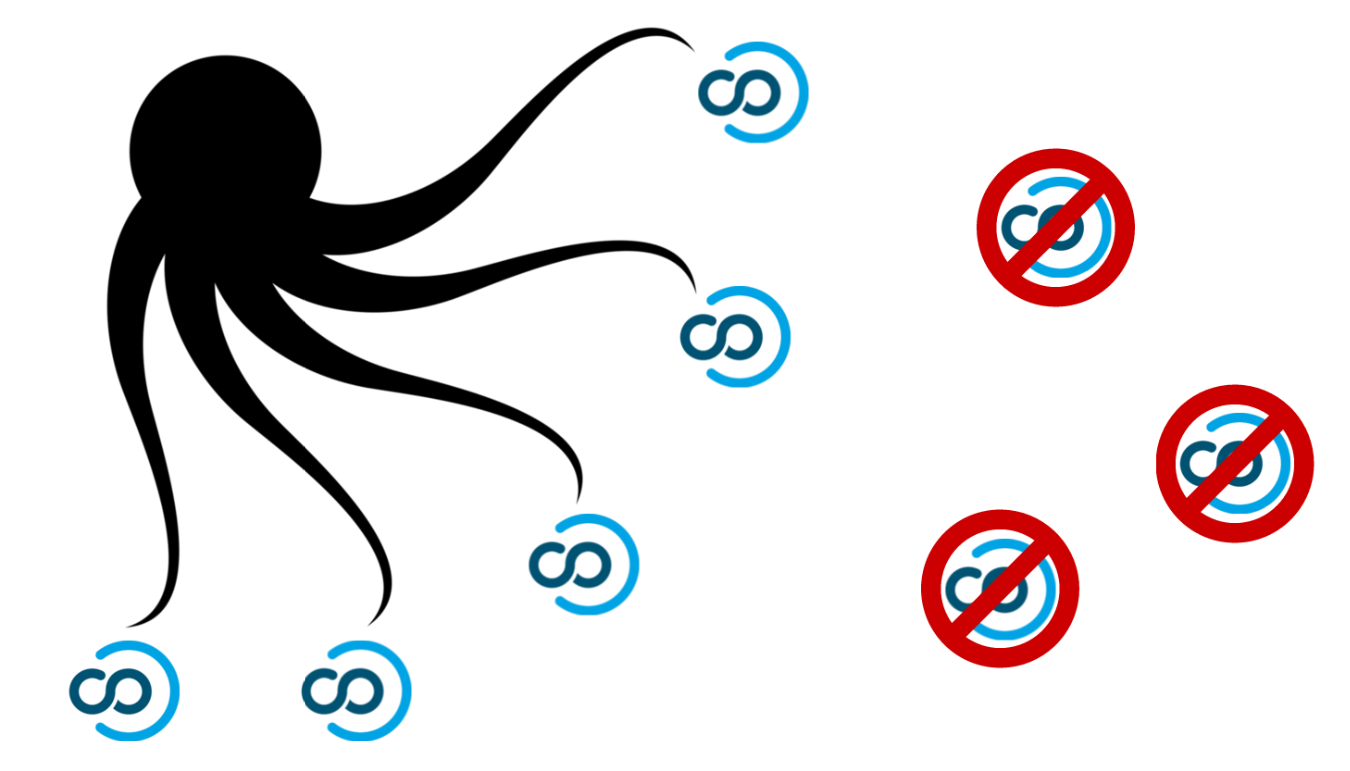
\includegraphics[scale=0.6]{cephalopod.png}
		\end{center}
		\caption[Stilizzazione di Cephalopod]{Stilizzazione di Cephalopod (fonte \cite{papini:kt}).}
		\label{fig:cephalopod}
	\end{figure}
	
	In Figura \ref{fig:cephalopod} possiamo vedere la stilizzazione dell'applicazione Cephalopod la quale, tramite ogni ``tentacolo'', raccoglie informazioni da ogni diversa istanza di Indico escludendo, ovviamente, quelle istanze che hanno scelto di non partecipare a quest'iniziativa di raccolta dati.
    
    \section{Caratteristiche principali} \label{sec:it;caratteristiche principali}
    
        Cephalopod è un'applicazione web basata su Flask che permette la registrazione di utenti (ovvero gli amministratori di Cephalopod e idealmente i principali sviluppatori dell'applicazione tracciata). Gli amministratori registrati potranno, tramite una semplice interfaccia web, accedere alla lista delle istanze tracciate, tramite la quale si accede alla pagina di gestione di ogni singola istanza, oppure alla pagina di statistiche, dove vengono rappresentate in forma grafica tutte le informazioni necessarie agli amministratori per prendere decisioni.
        
        In questa Sezione verranno descritte le principali caratteristiche di Cephalopod, nonché alcune istruzioni su come utilizzarlo.
        
        \subsection{Installazione e configurazione} \label{subsec:it;cp;installazione_configurazione}
        
            Per installare Cephalopod è necessario, innanzitutto, clonare il repository GitHub sul quale è archiviato il codice sorgente di Cephalopod e quindi posizionarsi nella cartella principale del codice. Per fare questo basta eseguire i seguenti due comandi da linea di comando:
            
            \begin{center}
                \begin{lstlisting}[language=bash, gobble=18]
                    $ git clone https://github.com/indico/cephalopod.git
                    $ cd cephalopod
                \end{lstlisting}
                \captionsetup{textformat=empty,labelformat=empty} \vspace{-2em}
                \captionof{lstlisting}[\bash{clone} del codice di Cephalopod]{Comando di \bash{clone} per ottenere il codice sorgente di Cephalopod.}
            \end{center}
            
            Una volta clonato con successo il repository del codice sorgente di Cephalopod, si può procedere con l'installazione. Per installare Cephalopod, si hanno due scelte. La prima (consigliata) prevede di installare Cephalopod all'interno di un ambiente virtuale Python dedicato, eseguendo le seguenti istruzioni:
            
            \begin{center}
                \begin{lstlisting}[language=bash, gobble=18]
                    $ virtualenv env
                    $ . env/bin/activate
                    $ pip install -r requirements.txt
                \end{lstlisting}
                \captionsetup{textformat=empty,labelformat=empty} \vspace{-2em}
                \captionof{lstlisting}[Installazione di Cephalopod (virtualenv)]{Installazione di Cephalopod in un ambiente virtuale dedicato.}
            \end{center}
            
            Altrimenti si può scegliere di installare Cephalopod direttamente per l'utente corrente. Per fare questo basterà eseguire il seguente comando:
            
            \begin{center}
                \begin{lstlisting}[language=bash, gobble=18]
                    $ python setup.py install
                \end{lstlisting}
                \captionsetup{textformat=empty,labelformat=empty} \vspace{-2em}
                \captionof{lstlisting}[Installazione di Cephalopod (globale)]{Installazione di Cephalopod nell'ambiente globale per l'utente corrente.}
            \end{center}
            
            Una volta terminata l'installazione di Cephalopod tramite una delle due modalità sopra esposte, si deve procedere con alcune fasi di configurazione, prima di poter iniziare ad utilizzare l'applicazione.
            Cephalopod utilizza un file di configurazione denominato \bash{settings.cfg}, all'interno della cartella \bash{cephalopod/}. Inizialmente il file non è presente e dev'essere creato dall'utente per poter utilizzare il software. Tuttavia, nel codice sorgente, è stato incluso un file di configurazione di esempio, denominato \bash{settings.cfg.example}, sul quale ci si può basare come punto di partenza per configurare Cephalopod. A riguardo, un comando utile potrebbe essere il seguente, che permette di copiare le configurazioni d'esempio nel file di configurazioni vero e proprio:
            
            \begin{center}
                \begin{lstlisting}[language=bash, gobble=18]
                    $ cp cephalopod/settings.cfg.example cephalopod/settings.cfg
                \end{lstlisting}
                \captionsetup{textformat=empty,labelformat=empty} \vspace{-2em}
                \captionof{lstlisting}[Copia delle configurazioni di Cephalopod]{Copia delle configurazioni d'esempio di Cephalopod come base di partenza.}
            \end{center}
            
            Bisogna tener presente, in generale quando si personalizza il file di configurazione, che esso deve essere scritto rispettando una corretta sintassi Python. Di seguito mostriamo la struttura del file di configurazione d'esempio:
            
            \begin{center}
                \begin{lstlisting}[language=python, gobble=18]
                    # Core settings
                    BABEL_DEFAULT_TIMEZONE = "UTC"
                    BABEL_DEFAULT_LOCALE = "en_GB"
                    ASSETS_DEBUG = False
                    SECRET_KEY = ''
                    APP_NAME = 'Cephalopod'
                    CRAWLING_ENDPOINTS = [
                        {
                            'url': '/example/endpoint',
                            'headers': {'Accept': 'application/json'}
                        },
                        {
                            'url': '/another/example/endpoint'
                        }
                    ]
                    CRAWLED_FIELDS_SETTINGS = {
                        'example_field': {
                            'label': 'The Example Field!',
                            'chart': True,
                            'chart_type': 'line',
                            'aggregation': 'sum',
                            'chart_aggregation': 'avg',
                            'chart_aggregate_by': 'another_example_field'
                        },
                        'example_field_2': {
                            'chart': True,
                            'chart_type': 'pie',
                            'chart_aggregation': 'avg',
                            'chart_aggregate_by': 'country'
                        }
                    }
                    
                    # Database settings
                    SQLALCHEMY_DATABASE_URI = 'postgresql:///cephalopod'
                    
                    # Celery settings
                    CELERY_BROKER_URL = 'redis://127.0.0.1:6379/0'
                    from datetime import timedelta
                    CELERYBEAT_SCHEDULE = {
                        'crawl-everything': {
                            'task': 'cephalopod.crawler.crawl_all',
                            'schedule': timedelta(days=1)
                        }
                    }
                \end{lstlisting}
                \captionsetup{textformat=empty,labelformat=empty} \vspace{-2em}
                \captionof{lstlisting}[Configurazioni d'esempio di Cephalopod]{Struttura del file di configurazione d'esempio per Cephalopod.}
            \end{center}
            
            La prima modifica necessaria al file di configurazione consiste nell'impostare il campo \python{SECRET_KEY} (utilizzato da Flask): basta aggiungere una parola chiave o una stringa alfanumerica casuale. Dopodiché si possono impostare i campi \python{BABEL_DEFAULT_TIMEZONE} e \python{BABEL_DEFAULT_LOCALE} che determinano, rispettivamente, in quale fuso orario e quale formato mostrare l'orario all'interno del software (di default sono \python{UTC} e \python{en_GB}, rispettivamente). Infine si può impostare il nome dell'applicazione che vogliamo tracciare (ad esempio Indico) tramite il campo \python{APP_NAME}.
            
            Riguardo ai restanti campi di configurazione, parleremo dei \textit{crawled field} (traducibili come ``campi estratti'' in italiano) qui di seguito, mentre tratteremo gli altri campi in Sezione \ref{sec:it;dettagli_implementativi}, quando analizzeremo Cephalopod dal punto di vista implementativo.
            
        \subsection{Non solo Indico} \label{sec:it;cp;non_solo_indico}
        
            Una delle caratteristiche centrali di Cephalopod è che, sebbene sia stato sviluppato con il fine principale di essere utilizzato per tracciare le istanze di Indico, esso è stato scritto in modo da poter funzionare per una generica applicazione web. Infatti Indico non è la sola applicazione web sviluppata e gestita all'interno del \ac{CERN}. Un esempio è Invenio\footnote{\url{http://invenio-software.org/}.}, un software, come Indico, open source che gestisce tutta la documentazione informatizzata al \ac{CERN} e funge da libreria digitale.
            
            Alcuni parametri del file \bash{settings.cfg}, come \python{APP_NAME} o \python{CRAWLING_END}- \python{POINTS}, servono proprio a definire quale applicazione deve tracciare Cephalopod e come deve farlo. \python{APP_NAME}, ad esempio, serve a definire il nome dell'applicazione tracciata (``Indico'', ad esempio) mentre \python{CRAWLING_ENDPOINTS} serve a definire come Cephalopod deve comunicare con le istanze da tracciare, come vedremo meglio in Sezione \ref{sec:it;dettagli_implementativi}. L'aggiunta di questo tipo di opzioni ha sicuramente reso lo sviluppo di Cephalopod più complesso ma ha anche permesso a Cephalopod di essere un'applicazione modulare e generalizzata, utilizzabile da una qualsiasi applicazione web. Inoltre, come vedremo successivamente, sarà anche possibile definire dei campi, che Cephalopod potrà estrarre, personalizzati e specifici per il tipo di applicazione tracciata. Indico, ad esempio, potrebbe aver bisogno di estrarre il numero di eventi in una certa istanza, mentre Invenio il numero di documenti presenti nella libreria.
            
            Chiaramente, Cephalopod non può tracciare un'applicazione che non sia stata prima adattata ad essere tracciata da Cephalopod, ovvero a comunicare con esso. In particolare, come vedremo meglio all'interno delle Sezioni \ref{sec:it;dettagli_implementativi} e \ref{sec:it;adattamento_indico}, un'applicazione dovrà implementare degli endpoint, ovvero dei particolari indirizzi tramite i quali Cephalopod può estrarre i dati. In Sezione \ref{sec:it;adattamento_indico} vedremo come questa implementazione è avvenuta nel caso specifico di Indico.
            
            Quindi, ricapitolando, Cephalopod è indirizzato a tutti gli sviluppatori di una generica applicazione web della quale sono interessati tracciarne le istanze ed il loro utilizzo nel mondo. Uno sviluppatore, dopo aver installato e configurato appropriatamente Cephalopod, dovrà quindi occuparsi di implementare gli endpoint sull'applicazione stessa, in modo da permettere la corretta comunicazione tra applicazione e tracciatore.
            
        \subsection{Campi principali e campi estratti} \label{subsec:it;cp;campi_principali_campi_estratti}
        
            È chiaro a questo punto che la mansione principale di Cephalopod è quella di raccolta dati da ogni singola istanza dell'applicazione tracciata. Risulta lecito a questo punto chiedersi quali informazioni vengano raccolte da Cephalopod.
            Le informazioni raccolte si dividono in due gruppi: informazioni \textit{principali} ed informazioni \textit{estratte}.
            
            \paragraph{Campi principali}Le informazioni principali sono campi di base che è necessario raccogliere per ogni tipo di applicazione. I campi principali, in particolare, sono 6 e sono i seguenti:
            
            \begin{itemize}
                \item \textbf{Organisation}: contiene il nome dell'organizzazione nella quale è installata l'istanza dell'applicazione;
                \item \textbf{URL}: l'indirizzo alla pagina principale dell'istanza;
                \item \textbf{Contact name}: il nome del responsabile dell'istanza;
                \item \textbf{Email}: l'indirizzo email a cui è possibile raggiungere il responsabile;
                \item \textbf{UUID}: identificatore \acr{UUID} assegnato all'istanza in modo univoco;
                \item \textbf{Enabled}: indica se l'istanza ha attivato il servizio di tracciamento oppure no.
            \end{itemize}
            
            Questi campi sono essenziali per Cephalopod ed ogni istanza, se e quando attiva il sistema di tracciamento, dovrà assicurarsi di fornirli tutti.
            
            \paragraph{Campi estratti}I campi estratti (anche detti ``campi aggiuntivi''), invece, sono campi specificati dall'amministratore di Cephalopod e possono essere di svariata natura: per quanto riguarda Indico, ad esempio, si potrebbe pensare a raccogliere il numero di eventi totali, o il numero di utenti registrati, o ancora la versione di Python utilizzata per una determinata istanza o la versione di Indico installata. I campi estratti possono essere di molti tipi: numerici, testuali, booleani, ecc. Questi campi hanno il fine principale di andare a formare le statistiche, sulla base delle quali l'amministratore potrà fare delle analisi e prendere delle decisioni.
            
            Per comunicare a Cephalopod come trattare i campi estratti (e quanti e quali sono) si utilizza il campo \python{CRAWLED_FIELDS_SETTINGS} all'interno del file di configurazione \bash{settings.cfg}. In questo senso Cephalopod è un'applicazione modulare in quanto permette all'amministratore di specificare tutti i campi extra che desidera e di personalizzarne il trattamento senza bisogno di dover andare a modificare il codice sorgente di Cephalopod: tutto sarà gestibile dal file di configurazione, tramite il campo \python{CRAWLED_FIELDS_SETTINGS}.
            
            Entrando più nel dettaglio, il campo \python{CRAWLED_FIELDS_SETTINGS} dev'essere un dizionario Python, dove ogni elemento dev'essere indicizzato da un nome chiave che identifica il campo, il quale deve coincidere con il nome di un campo estratto dall'istanza (come vedremo meglio in Sezione \ref{sec:it;dettagli_implementativi}): ogni nome che non combacia verrà ignorato.
            
            Per ogni campo aggiuntivo sarà quindi possibile selezionare una serie di opzioni, riassunte qui di seguito:
            
            \begin{itemize}
                \item \python{label}: stringa che specifica come rappresentare il nome del campo all'interno di Cephalopod; se non specificato, il valore di default è dato dal nome del campo sostituendo uno spazio ad ogni simbolo di underscore (\python{_}) e rendendo maiuscola la prima lettera della prima parola;
                \item \python{chart}: valore booleano che specifica se quel campo verrà incluso o meno tra le statistiche; default \python{False};
                \item \python{chart_type}: se \python{chart} è impostato a \python{True}, allora specifica che tipo di grafico utilizzare per visualizzare le statistiche relative al campo; i valori accettati sono \python{'bar'}, per avere un grafico a barre verticali, \python{'line'}, per un grafico a linea, e \python{'pie'}, per un grafico a torta; default \python{'bar'};
                \item \python{aggregation}: se il campo non può essere visualizzato direttamente (ad esempio è una lista o un dizionario), si deve definire una funzione di aggregazione per poter associare un singolo valore al campo; al momento sono supportati soltanto campi numerici di questo tipo; le funzioni di aggregazione possono essere \python{None}, se nessuna aggregazione è necessaria, \python{'sum'}, per restituire la somma, \python{'avg'}, per restituire il valor medio, e \python{'min'} e \python{'max'}, per restituire, rispettivamente, valor minimo e massimo; default \python{None};
                \item \python{chart_aggregation}: opzione simile a \python{aggregation}, serve a specificare come aggregare i valori del campo per ogni categoria quando \python{chart} è \python{True}; valori possibili sono \python{'count'}, per mostrare il numero di istanze per ogni categoria, \python{'sum'}, \python{'avg'}, \python{'min'} e \python{'max'}; default \python{'count'};
                \item \python{chart_aggregate_by}: stringa che specifica rispetto a quale altro campo raggruppare il campo corrente nelle statistiche; i valori accettati sono il nome di uno qualsiasi degli altri campi estratti oppure \python{'country'}, per raggruppare i valori rispetto al paese dell'istanza; se \python{chart_aggregation} è impostato a \python{'count'}, allora questa opzione verrà ignorata; default \python{'country'}.
            \end{itemize}
            
            Mostriamo di seguito, un paio di esempi per rendere più chiaro come funziona la definizione di campi aggiuntivi. Come primo esempio prendiamo il caso di Indico e supponiamo di voler definire un campo che contiene la versione di Python utilizzata da ogni istanza. Chiamiamo questo campo \python{python_version}. Ci aspettiamo che i valori di questo campo siano stringhe, quindi non c'è bisogno di specificare alcuna funzione di aggregazione. Supponiamo poi di voler includere questo campo tra le statistiche, mostrando un grafico a barre che, per ogni versione Python utilizzata, indica quante istanze ne fanno uso. Quindi, seguendo le definizioni date prima, dovremmo avere \python{chart} messo a \python{True}, \python{chart_type} settato su \python{'bar'} (o non incluso, essendo \python{'bar'} il valore di default) e \python{chart_aggregation} impostato a \python{'count'}. Il risultato è il seguente frammento di codice Python del file di configurazione:
            
            \begin{center}
                \begin{lstlisting}[language=python, gobble=18]
                    CRAWLED_FIELDS_SETTINGS = {
                        'python_version': {
                            'label': 'Python version',
                            'chart': True,
                            'chart_type': 'bar',
                            'chart_aggregation': 'count'
                        }
                    }
                \end{lstlisting}
                \captionsetup{textformat=empty,labelformat=empty} \vspace{-2em}
                \captionof{lstlisting}[Esempio di campo aggiuntivo (\python{python_version})]{Esempio di configurazione del campo aggiuntivo \python{python_version}.}
            \end{center}
            
            Se, quindi, volessimo rappresentare, tramite grafico a linea, anche il numero medio di eventi totali in ogni istanza che utilizza una determinata versione di Python, si potrebbe utilizzare la seguente configurazione:
            
            \begin{center}
                \begin{lstlisting}[language=python, gobble=18]
                    CRAWLED_FIELDS_SETTINGS = {
                        'python_version': {
                            'label': 'Python version',
                            'chart': True,
                            'chart_type': 'bar',
                            'chart_aggregation': 'count'
                        },
                        'events': {
                            'label': 'Events',
                            'chart': True,
                            'aggregation': 'sum',
                            'chart_type': 'line',
                            'chart_aggregation': 'avg',
                            'chart_aggregate_by': 'python_version'
                        }
                    }
                \end{lstlisting}
                \captionsetup{textformat=empty,labelformat=empty} \vspace{-2em}
                \captionof{lstlisting}[Esempio di campo aggiuntivo (\python{events})]{Esempio di configurazione del campo aggiuntivo \python{events}.}
            \end{center}
            
            In quest'ultimo esempio, si aggregano gli eventi tramite somma in quanto Indico raccoglie il numero di eventi diviso per categoria (quindi avremo un dizionario) e si richiede il numero totale di eventi. Impostando invece \python{chart_aggregation} a \python{'avg'} indichiamo a Cephalopod di mostrare, per ogni versione Python, il numero medio di eventi (totali), ovvero di fare la media tra il numero di eventi totali di ogni istanza che utilizza la stessa versione di Python.
            
            Per avere un'idea di come potrebbero apparire queste due configurazioni d'esempio, si veda la Figura \ref{fig:statistics_custom} a pagina \pageref{fig:statistics_custom}.
    
        \subsection{Interfaccia web} \label{subsec:it;cp;interfaccia_web}
        
            Parliamo adesso di com'è strutturata l'interfaccia web tramite la quale gli amministratori utilizzano Cephalopod. La struttura dell'applicazione è molto semplice ed è divisa, principalmente, in 4 sezioni: la pagina principale, la lista delle istanze, la pagina di gestione e dei dettagli di un'istanza e la pagina delle statistiche.
            
            \paragraph{Pagina principale e dettagli}La pagina principale viene utilizzata soltanto per effettuare il login e per accedere alle altre sezioni dell'applicazione. Per il resto, la pagina è piuttosto vuota e non presenta particolari funzionalità. Infatti è stata pensata come semplice punto di appoggio per eseguire il login e poi spostarsi sulle altre sezioni.
            
            Degna di nota sono anche la barra principale e le \textit{breadcrumbs} (``briciole di pane'' in italiano). La barra principale, posta in alto, è una barra reattiva (\textit{responsive}, in inglese), ovvero che si adatta alla larghezza dello schermo e, se troppo piccolo, si trasforma in un pulsante tramite il quale le varie voci vengono visualizzate in un apposito menu a tendina. Sulla destra della barra è stato posizionato il nome dell'utente attualmente loggato ed un pulsante per effettuare il logout. Le breadcrumbs, invece, sono poste subito sotto la barra del menu e permettono di sapere in ogni momento in che posizione dell'applicazione ci troviamo e di poter navigare velocemente da una pagina all'altra. Per garantire una maggior semplicità di navigazione, sia la barra del menu che le breadcrumbs sono state fissate sempre in alto in primo piano, sia cambiando pagina che scorrendo verso il basso. In Figura \ref{fig:menu_bar} si può vedere come appaiono la barra del menu e le breadcrumbs.
            
        	\begin{figure}[h!]
        		\begin{center}
        			
\includegraphics[scale=0.55]{menu_bar.png}
        		\end{center}
        		\caption[Barra del menu e breadcrumbs]{Barra del menu e breadcrumbs in Cephalopod.}
        		\label{fig:menu_bar}
        	\end{figure}
            
            \paragraph{Lista delle istanze}La pagina della lista delle istanze registrate, denominata \textit{server list}, serve invece a fornire a colpo d'occhio la situazione delle istanze attive al momento. In questa pagina si trova una lista delle istanze registrate, al momento o in passato, posizionata al centro. Per ogni voce sono indicati il nome dell'istanza, l'indirizzo e la data dell'ultima volta in cui sono stati aggiornati i dati. In Figura \ref{fig:server_list} possiamo vedere un esempio della pagina della lista delle istanze\footnote{Si faccia attenzione che in quest'immagine, come in tutte le altre presenti all'interno di questo capitolo, i dati presenti sono del tutto fittizi e creati ad-hoc al solo scopo illustrativo, in quanto Cephalopod non è ancora stato rilasciato e non è ancora in utilizzo, né al \ac{CERN} né altrove.}.
            
        	\begin{figure}[h!]
        		\begin{center}
        			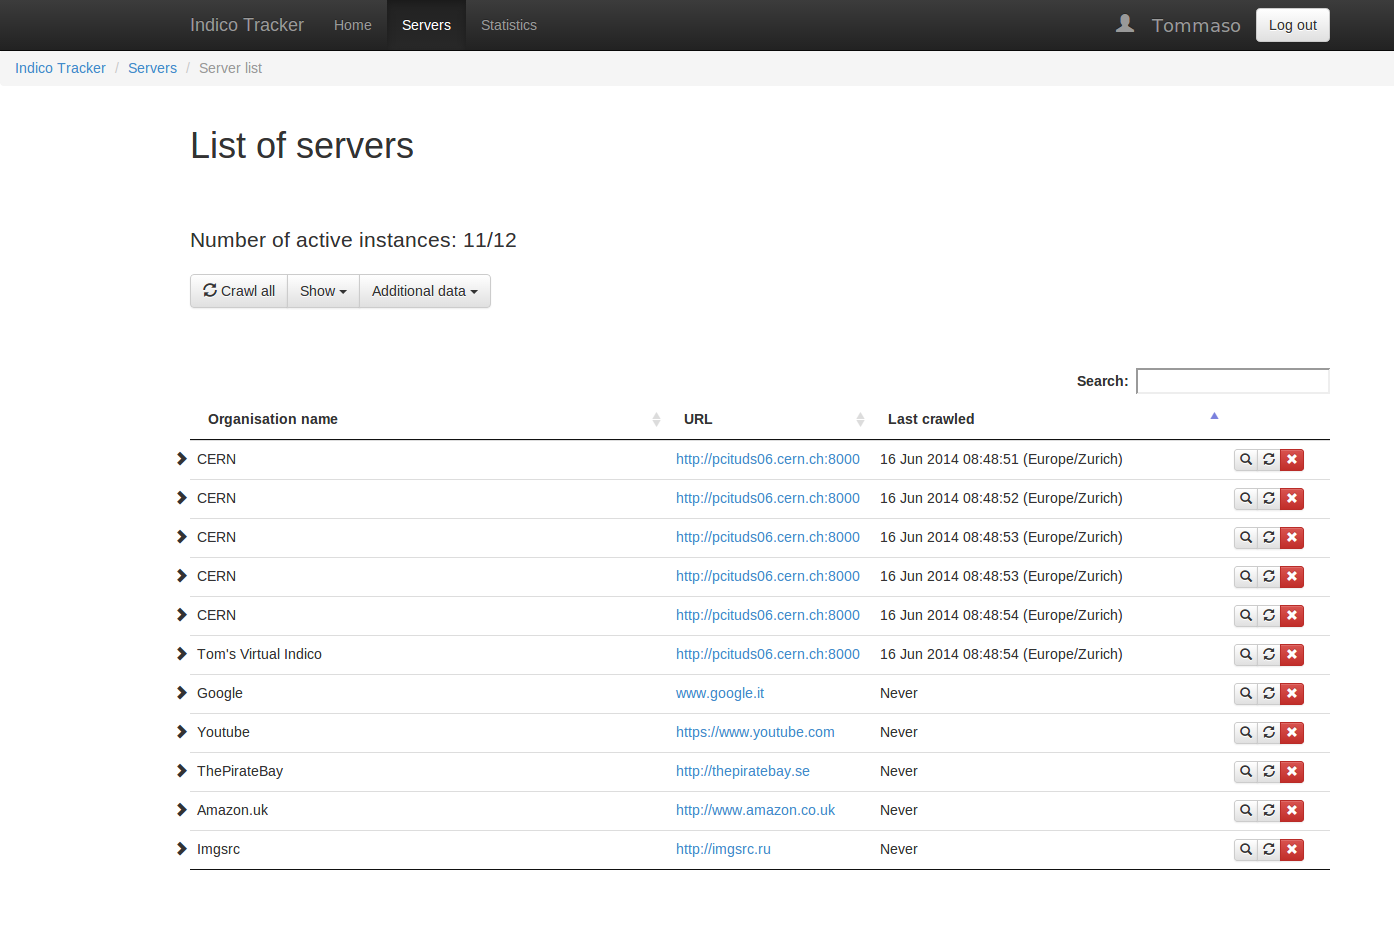
\includegraphics[scale=0.55]{server_list.png}
        		\end{center}
        		\caption[Lista delle istanze]{Pagina della lista delle istanze in Cephalopod.}
        		\label{fig:server_list}
        	\end{figure}
        	
        	Possiamo notare che per ogni istanza sono presenti tre pulsanti: il primo, indicato da una clessidra, serve ad aprire una nuova pagina, dedicata alla gestione di quell'istanza; il secondo, indicato dal simbolo di aggiornamento (o refresh), avvia il processo di aggiornamento dei dati (principali e aggiuntivi) per quella particolare istanza; il terzo invece, indicato da una croce, permette di eliminare quell'istanza dalla lista. La freccia alla sinistra del nome di ogni istanza serve ad espandere i dettagli di quell'istanza, aprendo un riquadro a tendina sotto alla voce, dove vengono riassunti i valori di tutti gli altri campi non mostrati. In alto si possono notare tre bottoni: il primo (``Crawl all'') serve a forzare l'aggiornamento dei dati per tutte le istanze attive; il secondo (``Show'') apre un menu a tendina tramite il quale si possono selezionare quali istanze mostrare nella lista (attive, disattive o entrambe); il terzo (``Additional data'') serve invece ad includere direttamente su ogni riga i campi non mostrati inizialmente (senza bisogno di cliccare sulla freccia a sinistra di ogni voce), come possiamo vedere in Figura \ref{fig:server_list_additional_data}.
        	
        	\begin{figure}[h!]
        		\begin{center}
        			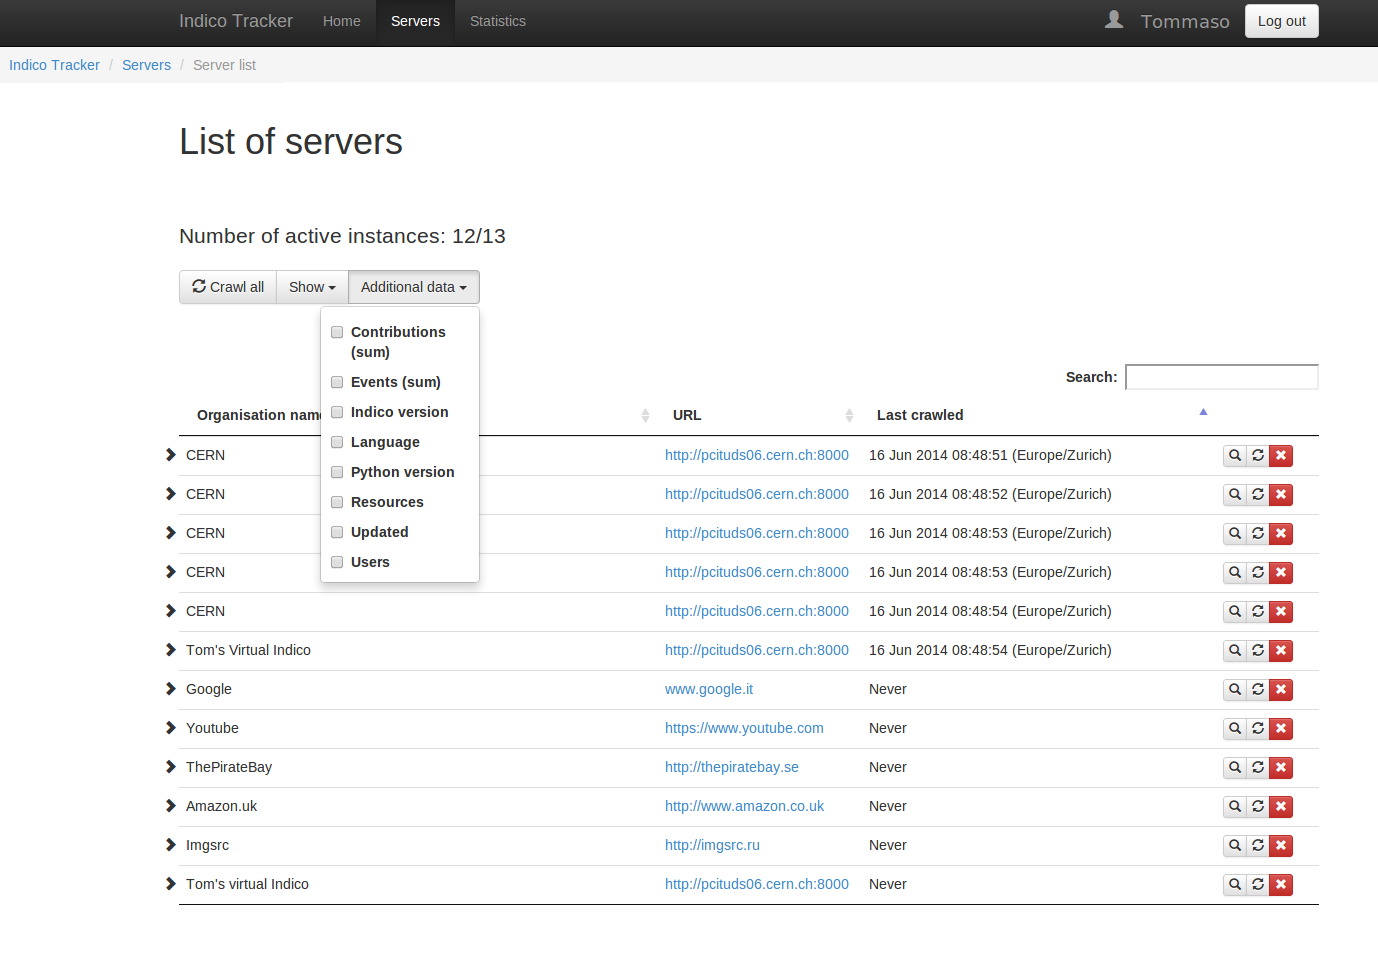
\includegraphics[scale=0.55]{server_list_additional_data.png}
        		\end{center}
        		\caption[Lista delle istanze (con menu a tendina aperto)]{Pagina della lista delle istanze in Cephalopod col menu a tendina ``Additional data'' aperto.}
        		\label{fig:server_list_additional_data}
        	\end{figure}
        	
        	Infine notiamo una barra di ricerca, in alto a destra, che permette di filtrare le istanze della lista in base a delle parole chiave, e delle piccole frecce accanto ad ogni colonna della lista, che permetto di ordinare la lista secondo quel determinato campo (ad esempio un amministratore potrebbe voler visualizzare la lista per ordine decrescente di numero totale di eventi).
        	
        	\paragraph{Dettagli di un'istanza}Se, dalla lista delle istanze, si clicca sul pulsante contrassegnato da una lente di ingrandimento, si accede ad una pagina dedicata ai dettagli di quell'istanza. In Figura \ref{fig:server_management} possiamo vedere una schermata rappresentativa di come appare la pagina dei dettagli.
        	
        	\begin{figure}[h!]
        		\begin{center}
        			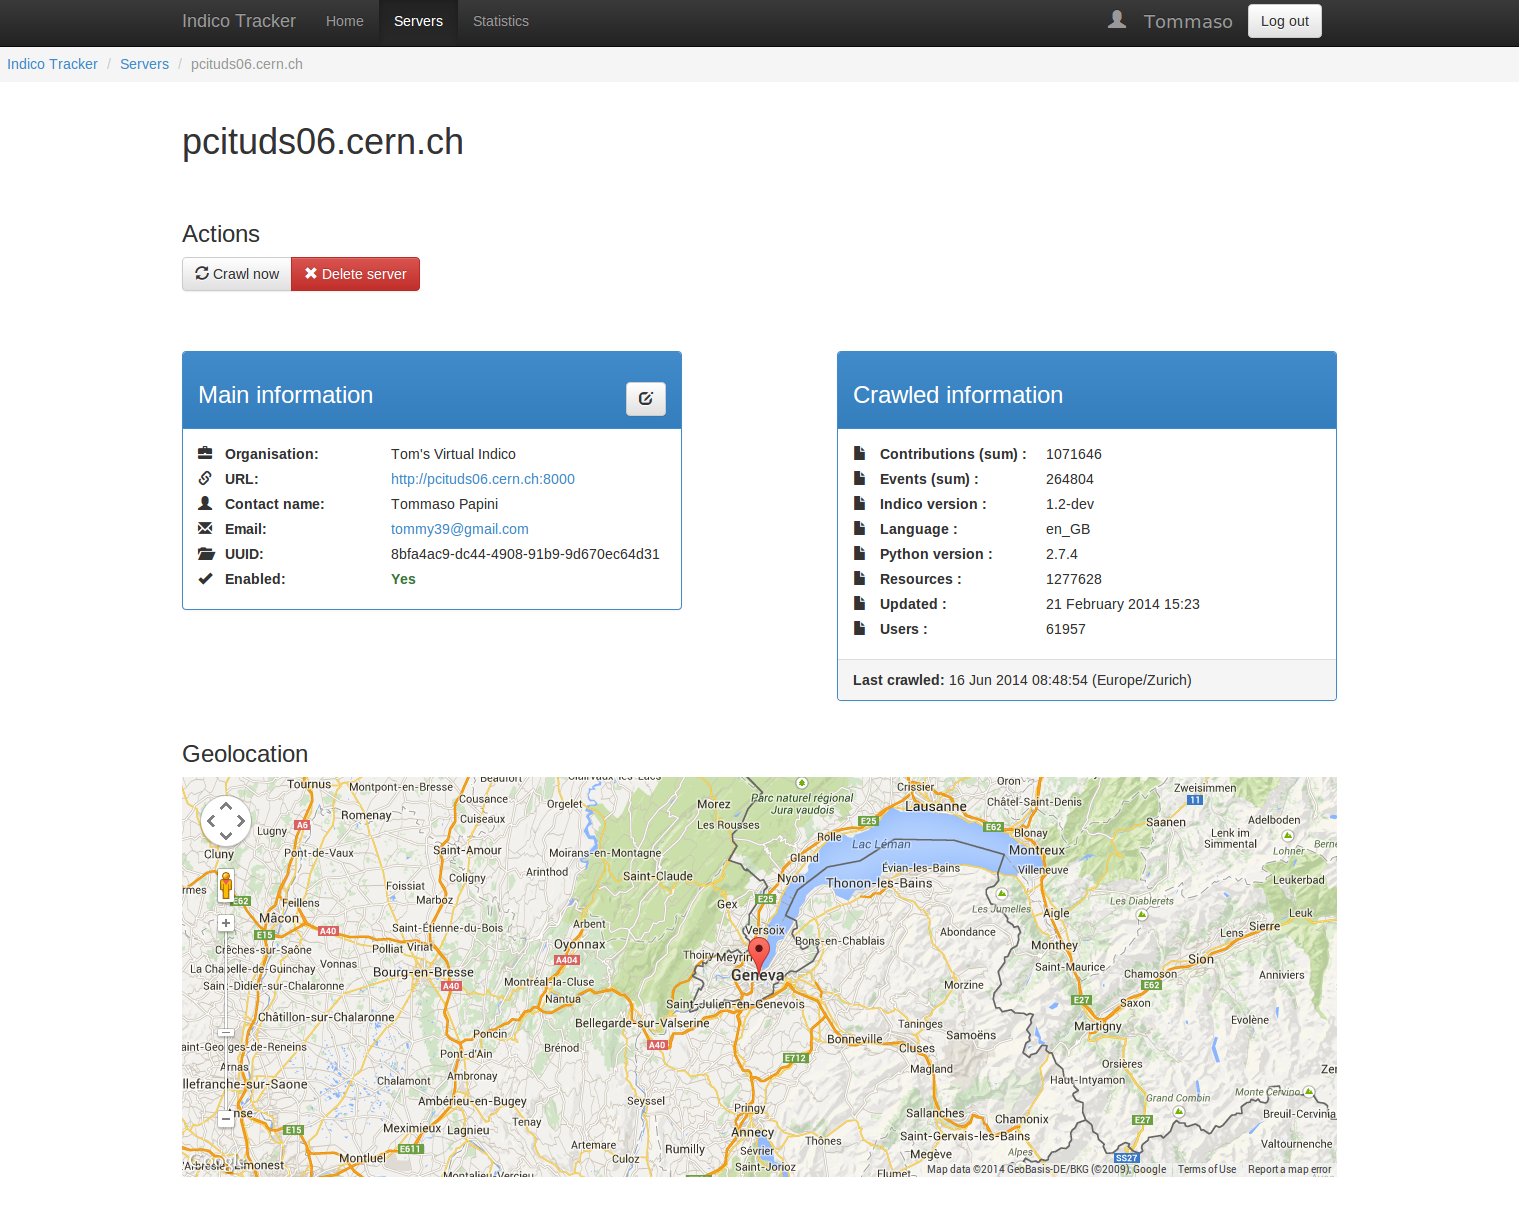
\includegraphics[scale=0.5]{server_management.png}
        		\end{center}
        		\caption[Dettagli di un'istanza]{Pagina dei dettagli e di gestione di un'istanza.}
        		\label{fig:server_management}
        	\end{figure}
        	
        	Analizziamo, adesso, la struttura della pagina. In alto troviamo l'indirizzo base dell'istanza, in qualità di titolo della pagina, e due bottoni di azione: ``Crawl now'', che forza la raccolta di informazioni per quell'istanza, e ``Delete server'', che invece la elimina dal database di Cephalopod.
        	
        	Subito sotto alle azioni troviamo due riquadri: ``Main information'' e ``Crawled information''. Il riquadro ``Main information'' raccoglie tutti i campi principali descritti prima, mostrandone il valore relativo a quell'istanza particolare. Il pulsante simile ad una penna che scrive posizionato accanto al titolo ``Main information'' serve per permettere all'amministratore di Cephalopod di modificare i campi principali per una determinata istanza, nel caso avessero bisogno di essere aggiornati: cliccandoci, il valore di ogni campo si trasformerà in un input field, dove sarà possibile inserire il valore aggiornato, oppure lasciarlo invariato, per poi cliccare su un bottone di salvataggio che comparirà durante la modifica. Nel riquadro ``Crawled information'' vengono invece raccolti tutti i dati estratti aggiuntivi, ovvero i campi definiti dall'amministratore di Cephalopod all'interno del file \bash{settings.cfg}. In fondo al riquadro, inoltre, verrà visualizzata l'ultima data in cui sono stati estratti i dati. Come possiamo vedere dall'esempio in Figura \ref{fig:server_management}, alcuni di questi dati possono essere di tipo numerico (numero di utenti, numero di risorse, ecc\dots) oppure di tipo testuale (come la lingua o la data di ultimo aggiornamento di Indico). Si può vedere inoltre che i dati aggregati, come il numero di eventi, sono affiancati, tra parentesi, dalla funzione di aggregazione scelta (nell'esempio abbiamo il numero totale di eventi, in quanto l'aggregazione è fatta tramite somma).
        	
        	Infine, in basso compare una mappa, che mostra la geolocalizzazione dell'istanza. Come vedremo meglio in Sezione \ref{sec:it;dettagli_implementativi}, la geolocalizzazione avviene in automatico sfruttando l'indirizzo \acr{IP} durante la fase di estrazione dei dati.
        	
        	\paragraph{Statistiche}La pagina delle statistiche è forse la pagina più importante per l'amministratore di Cephalopod in quanto raccoglie tutti i dati ottenuti dalle varie istanze e li presenta all'amministratore in forma grafica ed intuitiva, permettendo, a colpo d'occhio, di qual è la situazione delle istanze rispetto a certi aspetti di interesse.
        	
        	La prima parte della pagina è fissa ed è illustrata in Figura \ref{fig:statistics_main}.
        	
        	\begin{figure}[h!]
        		\begin{center}
        			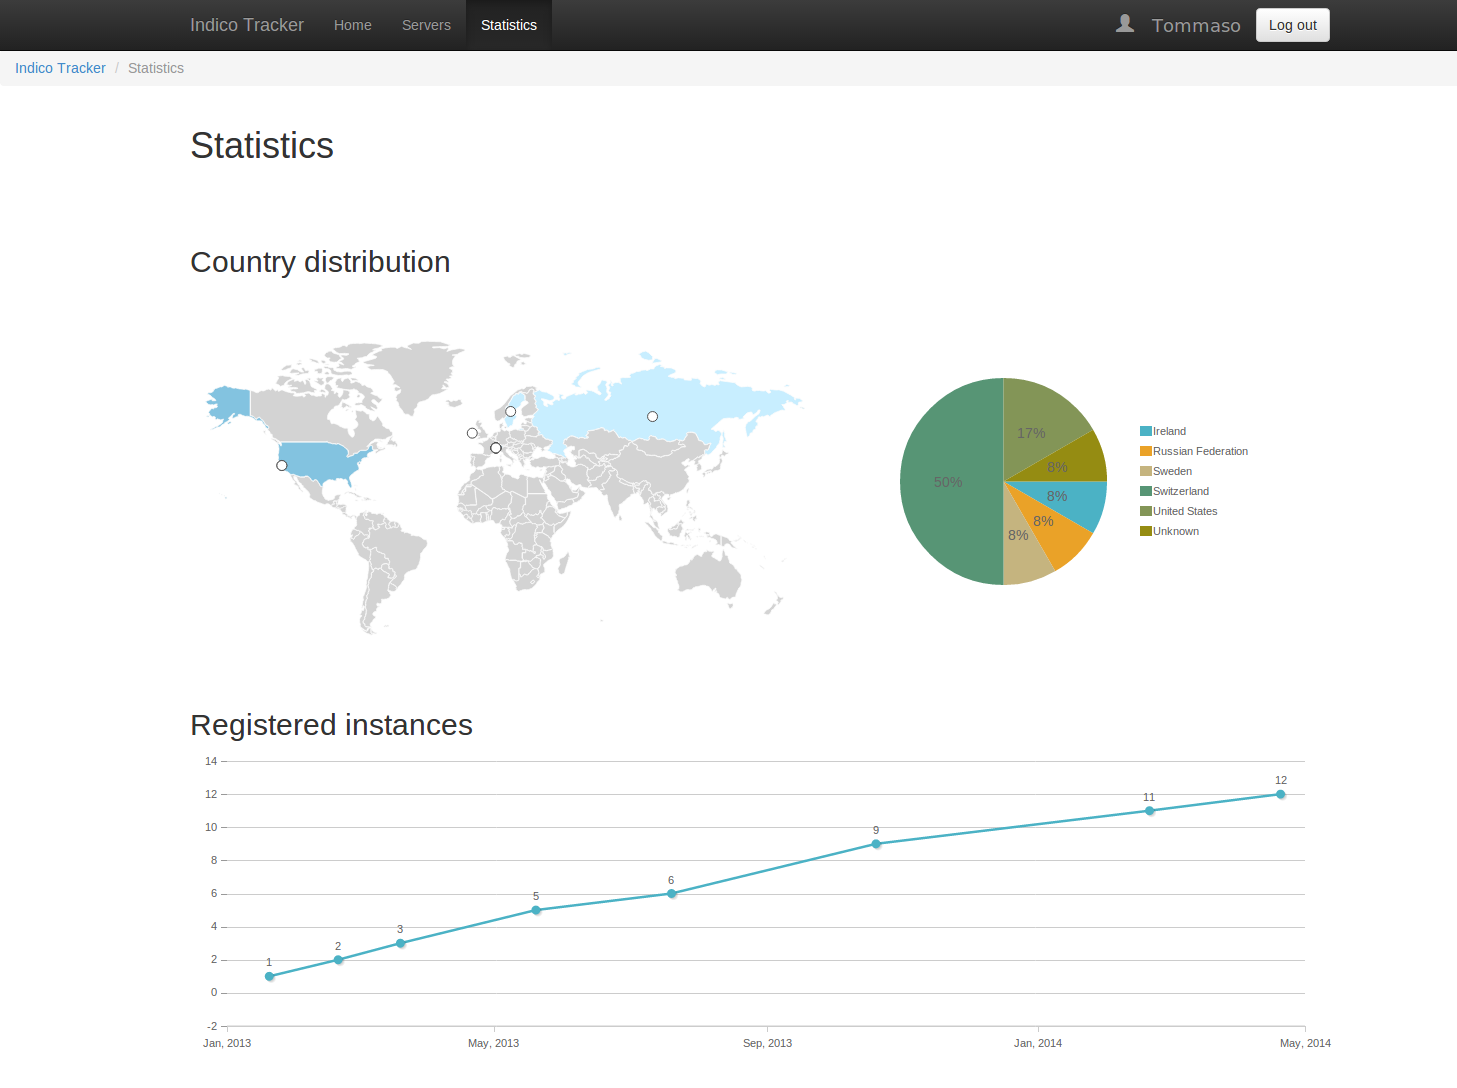
\includegraphics[scale=0.5]{statistics_main.png}
        		\end{center}
        		\caption[Statistiche principali]{Parte principale della pagina delle statistiche.}
        		\label{fig:statistics_main}
        	\end{figure}
        	
        	Nella parte superiore troviamo una mappa ed un grafico a torta che rappresentano la distribuzione delle istanze per paese. Nella mappa compare un puntino in corrispondenza di ogni istanza registrata e geolocalizzata correttamente e ogni stato viene colorato di una determinata sfumatura di blu oppure grigio, dove blu scuro indica un'alta concentrazione di istanze in quello stato, blu chiaro una bassa concentrazione e grigio indica nessuna istanza in quel determinato stato. Il grafico a torta serve invece a mostrare, a colpo d'occhio, la percentuale di istanze per ogni stato.
        	
        	Subito sotto alla distribuzione per paese, viene mostrato un grafico a linea dove si può vedere come si evolve il numero di istanze registrate a Cephalopod nel tempo.
        	
        	I grafici della distribuzione per paese e delle istanze registrate nel tempo sono sempre presenti nella pagina delle statistiche e non possono essere modificati. Subito sotto, invece, si sviluppa la parte dinamica della pagina, ovvero la parte dedicata alle statistiche definite dall'amministratore. In particolare, tutti i grafici che l'amministratore ha abilitato e configurato in \bash{settings.cfg} saranno visualizzati in questa pagina, in ordine di definizione, immediatamente sotto al grafico delle istanze registrate.
        	
        	A titolo d'esempio mostriamo alcuni grafici, in Figura \ref{fig:statistics_custom}, che mostrano diversi modi di definire delle statistiche sui vari campi aggiuntivi.
        	
        	\begin{figure}[h!]
        		\begin{center}
        			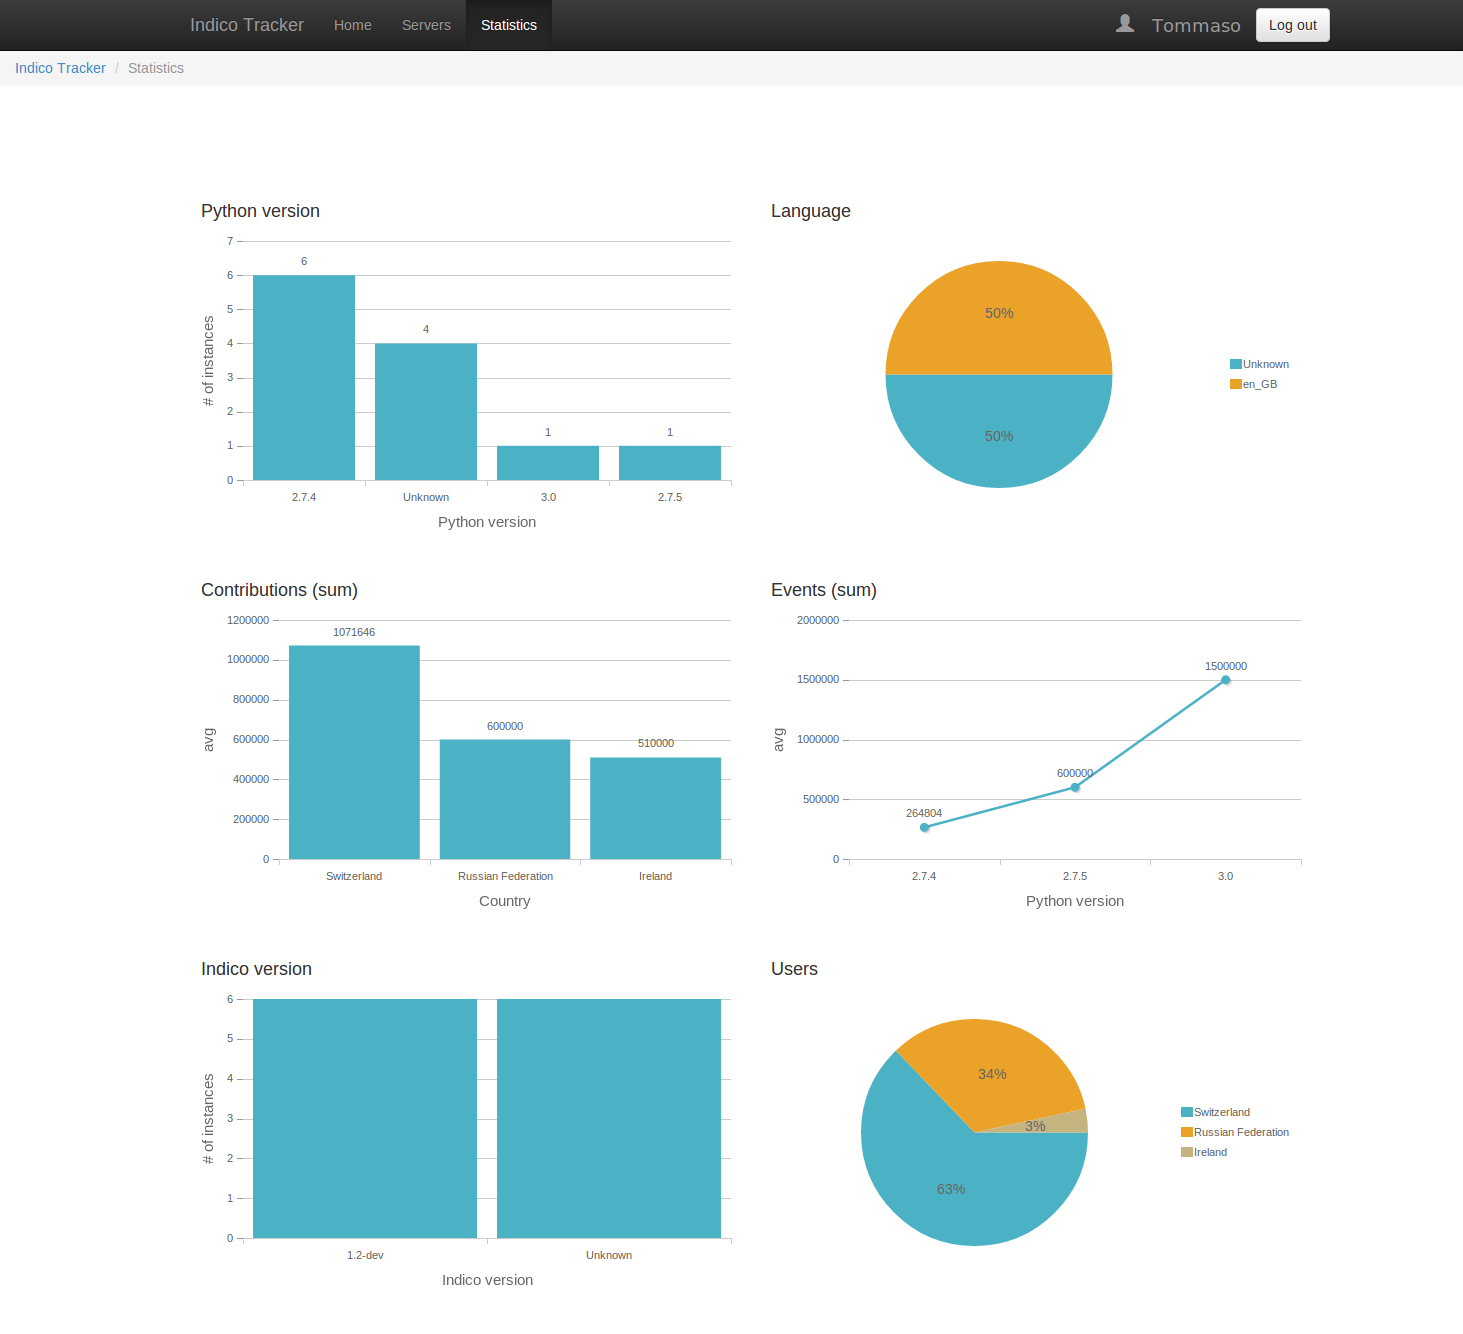
\includegraphics[scale=0.5]{statistics_custom.png}
        		\end{center}
        		\caption[Statistiche definite dall'amministratore]{Parte personalizzabile della pagina delle statistiche che contiene le statistiche definite dall'amministratore.}
        		\label{fig:statistics_custom}
        	\end{figure}
        	
        	In particolare, il primo ed il terzo grafico (partendo dall'alto a sinistra) in Figura \ref{fig:statistics_custom} sono il risultato delle configurazioni d'esempio viste all'interno della Sottosezione \ref{subsec:it;cp;campi_principali_campi_estratti}.
        
        \subsection{Scheduler} \label{subsec:it;cp;scheduler}
        
            Cephalopod utilizza Celery\footnote{\url{http://www.celeryproject.org/}.} come scheduler, ovvero come modulo che si occupa di gestire eventi periodici. Le impostazioni di Celery sono controllare interamente dal file di configurazioni \bash{settings.cfg}. Se, ad esempio, l'amministratore di Cephalopod volesse impostare l'estrazione dei dati da tutte le istanze in modo che venga eseguita in automatico ogni giorno, basterebbe includere il seguente frammento di codice all'interno di \bash{settings.cfg}:
            
            \begin{center}
                \begin{lstlisting}[language=python, gobble=18]
                    from datetime import timedelta
                    CELERYBEAT_SCHEDULE = {
                        'crawl-everything': {
                            'task': 'cephalopod.crawler.crawl_all',
                            'schedule': timedelta(days=1)
                        }
                    }
                \end{lstlisting}
                \captionsetup{textformat=empty,labelformat=empty} \vspace{-2em}
                \captionof{lstlisting}[Impostazioni di Celery (esempio)]{Esempio di impostazioni per Celery per estrarre tutte le istanze ogni giorno automaticamente.}
            \end{center}
            
            Il campo \python{task} serve a indicare che comando eseguire e dev'essere una qualsiasi funzione messa a disposizione da Cephalopod (in questo caso si richiama la funzione \python{crawl_all} del file \bash{crawler.py} all'interno della cartella \bash{cephalopod}). Nel campo \python{schedule} si deve invece indicare l'intervallo di tempo che deve passare tra due esecuzioni successive dello stesso comando (in questo esempio, un giorno).
        
        \subsection{Script di gestione} \label{subsec:it;cp;script_gestione}
        
            Abbiamo già mostrato come sia possibile, per un amministratore di Cephalopod, gestire e aggiornare le istanze tramite l'applicazione web stessa, o come sia possibile gestire le impostazioni, ad esempio delle statistiche, attraverso il file di configurazione \bash{settings.cfg}. Ci sono tuttavia alcune operazioni avanzate che, con questi due soli strumenti, non è possibile effettuare. Per dare all'amministratore, quindi, tutti gli strumenti necessari a gestire Cephalopod nel migliore dei modi è stato scritto uno script in python che esegue alcune operazioni da linea di comando.
            
            Per utilizzare lo script basta immettere, da linea di comando, il seguente codice, nel caso in cui si sia installato Cephalopod tramite \bash{setup.py}:
            
            \begin{center}
                \begin{lstlisting}[language=bash, gobble=18]
                    $ cephalopod <argomenti>
                \end{lstlisting}
                \captionsetup{textformat=empty,labelformat=empty} \vspace{-2em}
                \captionof{lstlisting}[Script di gestione (con \bash{setup.py})]{Invocazione dello script di gestione avendo installato Cephalopod con \bash{setup.py}.}
            \end{center}
            
            Altrimenti, basterà eseguire il seguente comando:
            
            \begin{center}
                \begin{lstlisting}[language=bash, gobble=18]
                    $ python manage.py <argomenti>
                \end{lstlisting}
                \captionsetup{textformat=empty,labelformat=empty} \vspace{-2em}
                \captionof{lstlisting}[Script di gestione]{Invocazione dello script di gestione.}
            \end{center}
            
            Gli argomenti che si possono passare allo script di gestione sono elencati di seguito:
            
            \begin{itemize}
                \item \bash{shell}: apre una shell Python interattiva all'interno del contesto dell'applicazione Flask;
                \item \bash{runserver}: avvia l'applicazione Flash che gestisce il web server di Cephalopod;
                \item \bash{db drop}: elimina tutte le tabelle del database;
                \item \bash{db create}: crea le tabelle del database;
                \item \bash{db recreate}: elimina tutte le tabelle del database e ne crea di nuove (equivalente a fare \bash{drop} e \bash{create});
                \item \bash{crawl [uuid]}: estrae i dati da una specifica istanza (se viene passato un \ac{UUID}), altrimenti tutte;
                \item \bash{create_usr usr pswd}: crea un nuovo utente con \bash{usr} come username e \bash{pswd} come password di accesso;
                \item runworker [concurrency]: avvia un processo Celery; \bash{concurrency} è un intero che indica con che grado di parallelismo far partire il processo.
            \end{itemize}
    
    \section{Dettagli implementativi} \label{sec:it;dettagli_implementativi}
    
        Dopo aver descritto le caratteristiche principali di Cephalopod, tra cui la sua struttura ed il suo utilizzo, entriamo adesso un po' più nel dettaglio, esaminando gli aspetti tecnici e implementativi del codice di Cephalopod.
        
        Come già detto, Cephalopod è un'applicazione web scritta in Python, basata su Flask e che utilizza elementi \ac{HTML} forniti da Twitter Bootstrap per ottenere un design moderno e reattivo.
        
        \subsection{Struttura del codice} \label{subsec:it;di;struttura_codice}
        
            I file principali del codice sorgente di Cephalopod sono tutti contenuti all'interno della cartella \bash{cephalopod/}. I file più importanti che troviamo in questa cartella sono \bash{settings.cfg}, \bash{manage.py}, \bash{factory.py} e \bash{crawler.py}.
            
            Del file di configurazione \bash{settings.cfg} abbiamo già ampiamente parlato nella Sezione precedente. Il file \bash{manager.py} è lo script di gestione di cui abbiamo parlato prima e contiene la definizione di tutti i comandi possibili descritti prima. \bash{factory.py} serve a definire le funzioni che istanziano una nuova applicazione Flask (quando si avvia il web server) o un nuovo processo Celery. Infine, \bash{crawler.py} definisce tutte le funzioni dedicate all'estrazione delle informazioni dalle istanze, come ad esempio la geolocalizzazione.
            
            Il codice di Cephalopod si sviluppa quindi all'interno di quattro cartelle principali: \bash{api/}, \bash{models/}, \bash{templates/} e \bash{webinterface/}, sempre all'interno della cartella \bash{cephalopod/}.
            
            La cartella \bash{api/} contiene il solo file \bash{instance.py}, dove vengono definite le \ac{API} messe a disposizione di Cephalopod. All'interno di \bash{models/} troviamo i due file, \bash{instance.py} e \bash{user.py}, che definiscono il tipo di oggetti che possiamo memorizzare all'interno del database. Dentro \bash{templates/} troviamo invece una serie di file, in formato \bash{.html}, che servono, appunto, da template per generare pagine dal contenuto dinamico. Infine la cartella \bash{webinterface/} contiene il solo file \bash{misc.py} dove si definiscono le varie pagine di Cephalopod, ovvero la struttura dell'applicazione.
            
        \subsection{Il Database} \label{subsec:it;di;database}
        
            Il database utilizzato da Cephalopod è PostgreSQL. Per poter utilizzare PostgreSQL all'interno di Cephalopod, che è un'applicazione scritta in Python, si è utilizzato il toolkit SQLAlchemy, che mette a disposizione molte funzioni utili per gestire il database.
            
            All'interno della cartella \bash{models} abbiamo i due file, \bash{instance.py} e \bash{user.py}, che definiscono il tipo di oggetti che si possono archiviare all'interno del database. \bash{instance.py} definisce una classe \python{Instance} che, intuitivamente, serve a memorizzare le informazioni di una specifica istanza, mentre \bash{user.py} definisce la classe \python{User}, che memorizza le informazioni di ogni utente.
            
            I campi della classe \python{Instance} sono:
            
            \begin{itemize}
                \item \python{id}: ID da utilizzare come chiave primaria;
                \item \python{uuid}: identificatore \ac{UUID} assegnato all'istanza;
                \item \python{enabled}: valore booleano che indica se l'istanza è abilitata o meno;
                \item \python{url}: l'\ac{URL} dell'istanza;
                \item \python{contact}: il nome della persona di riferimento;
                \item \python{email}: l'indirizzo email della persona di riferimento;
                \item \python{organisation}: nome dell'organizzazione nella quale è installata l'istanza;
                \item \python{crawl_date}: data dell'ultima estrazione di informazioni;
                \item \python{crawled_data}: i dati aggiuntivi raccolti;
                \item \python{geolocation}: informazioni sulla geolocalizzazione del server;
                \item \python{registration_date}: data di registrazione dell'istanza su Cephalopod.
            \end{itemize}
            
            I campi della classe \python{User} sono invece:
            
            \begin{itemize}
                \item \python{id}: come prima, rappresenta la chiave primaria nel database;
                \item \python{username}: username dell'utente;
                \item \python{password}: password scelta, memorizzata sotto cifratura;
                \item \python{registered_on}: data di registrazione dell'utente.
            \end{itemize}
            
            La definizione della classe \python{User} è, escluse le funzioni accessorie, la seguente:
            
            \begin{center}
                \begin{lstlisting}[language=python, gobble=18]
                    class User(db.Model):
                        __tablename__ = "users"
                        id = db.Column('user_id', db.Integer, primary_key=True)
                        username = db.Column('username', db.String, unique=True, index=True)
                        password = db.Column('password', db.String)
                        registered_on = db.Column('registered_on', db.DateTime)
                \end{lstlisting}
                \captionsetup{textformat=empty,labelformat=empty} \vspace{-2em}
                \captionof{lstlisting}[Definizione della classe \python{User}]{Definizione della classe di oggetti \python{User} per il database.}
            \end{center}
            
            SQLAlchemy mette a disposizione molti tipi di dato tra cui scegliere, come \python{db.String} per le stringhe o \python{db.DateTime} per le date. Tuttavia può capitare di dover includere un campo di un tipo non supportato, nel qual caso è necessario definire prima il tipo di dato e come esso si comporta. In Cephalopod questo è stato necessario per i campi \python{crawled_data} e \python{geolocation} della classe \python{Instance} in quanto essi devono memorizzare strutture dati complesse, in particolare dizionari di tipo \ac{JSON}, e questo tipo non viene offerto da SQLAlchemy. Per aggiungere la possibilità di memorizzare dizionari \ac{JSON} all'interno del database, si è quindi aggiunta la seguente definizione (fonte \cite{sqlalchemy:custom}):
            
            \begin{center}
                \begin{lstlisting}[language=python, gobble=18]
                    class JSONEncodedDict(TypeDecorator):
                    
                        impl = VARCHAR
                    
                        def process_bind_param(self, value, dialect):
                            if value is not None:
                                value = json.dumps(value)
                            return value
                    
                        def process_result_value(self, value, dialect):
                            if value is not None:
                                value = json.loads(value)
                            return value
                \end{lstlisting}
                \captionsetup{textformat=empty,labelformat=empty} \vspace{-2em}
                \captionof{lstlisting}[Definizione di una classe JSON per SQLAlchemy]{Definizione della classe per il supporto di dizionari JSON utilizzando SQLAlchemy.}
            \end{center}
            
            Quindi, la definizione dei campi \python{crawled_data} e \python{geolocation} risulta essere la seguente:
            
            \begin{center}
                \begin{lstlisting}[language=python, gobble=18]
                    crawled_data = db.Column(JSONEncodedDict)
                    geolocation = db.Column(JSONEncodedDict)
                \end{lstlisting}
                \captionsetup{textformat=empty,labelformat=empty} \vspace{-2em}
                \captionof{lstlisting}[\python{crawled_data} e \python{geolocation}]{Definizione dei campi \python{crawled_data} e \python{geolocation}.}
            \end{center}
            
            SQLAlchemy mette a disposizione anche altre funzioni molto utili, ad esempio \python{db.drop_all()}, che elimina tutte le tabelle presenti, \python{db.create_all()}, che crea le tabelle, e \python{db.session.commit()}, che aggiorna il database con le modifiche fatte.
    
        \subsection{Endpoint ed API} \label{subsec:it;di;endpoint_API}
        
            Parliamo adesso di endpoint e di \ac{API}. Di fatto, quando parliamo di applicazioni web, endpoint ed \ac{API} significano la stessa cosa. All'interno di Cephalopod, tuttavia, questi due termini vengono utilizzati per esprimere due cose distinte. Con endpoint si intende gli \ac{URL} che l'applicazione che si vuole tracciare tramite Cephalopod deve implementare per permettere a Cephalopod di estrarre i dati voluti. Con \ac{API} si intendono invece gli \ac{URL} messi a disposizione da Cephalopod per permettere alle varie istanze di comunicare con Cephalopod. Detto questo, \ac{URL} endpoint ed \ac{API} esprimono entrambi il concetto di \ac{URL} tramite il quale si accede a un servizio.
            
            Gli endpoint tramite i quali Cephalopod può accedere ai dati di una certa istanza devono essere definiti in \bash{settings.cfg} ed in particolare nel campo \python{CRAWLING_ENDPOINTS}. \python{CRAWLING_ENDPOINTS} è una lista dove ogni elemento corrisponde ad un endpoint. Ogni elemento della lista, a sua volta, dovrà essere un dizionario Python contenente il campo \python{url}, dove si specifica l'endpoint, ed eventualmente un campo \python{headers}, che deve contenere un dizionario Python con le opzioni da utilizzare quando si estraggono informazioni da quello specifico endpoint. La stringa specificata nel campo \python{url} viene concatenata in fondo all'\ac{URL} di base di ogni istanza per formare l'\ac{URL} vero e proprio da cui estrarre i dati. Per questo motivo viene chiamato ``endpoint'': in quanto si specifica soltanto la parte finale dell'\ac{URL}.
            
            Ovviamente ogni applicazione che si vuole tracciare con Cephalopod deve implementare questi endpoint, per permettere a Cephalopod di comunicare con essa. Questo, chiaramente, dipende da applicazione a applicazione ed ogni sviluppatore ha il compito di implementare le proprie \ac{API} per permettere alla propria applicazione di comunicare con Cephalopod. In Sezione \ref{sec:it;adattamento_indico} vedremo l'implementazione di questi endpoint nel caso di Indico.
            
            Le \ac{API} messe a disposizione da Cephalopod per permettere alle istanze di comunicare con esso definiscono invece tre endpoint distinti, ognuno con una diversa funzione. Ogni \ac{API} è caratterizzata, quindi, da un endpoint, che rappresenta la parte finale dell'\ac{URL} al quale si può raggiungere Cephalopod, da un tipo di richiesta \ac{HTTP}, da dei dati da inviare con la richiesta e da una risposta che si può ricevere dopo aver inviato la richiesta. Di seguito si descrivono le tre \ac{API} fornite: 
            
            \begin{itemize}
                \item \textbf{Create instance}: questa \ac{API} è utilizzata per inserire una nuova istanza nel database di Cephalopod.
                    \begin{itemize}
                        \item \textit{Endpoint}: \html{/instance/};
                        \item \textit{Tipo di richiesta}: \html{POST};
                        \item \textit{Dati}: l'\ac{URL} del server dell'istanza, nome ed email della persona di riferimento e nome dell'organizzazione;
                        \item \textit{Risposta}: il nuovo \ac{UUID} assegnato all'istanza.
                    \end{itemize}
                \item \textbf{Update instance}: utilizzata per aggiornare i dati dell'istanza ogni qualvolta questi venissero cambiati (include il caso in cui si l'amministratore dell'istanza decida di abilitare/disabilitare il servizio di tracciamento).
                    \begin{itemize}
                        \item \textit{Endpoint}: \html{/instance/<uuid>};
                        \item \textit{Tipo di richiesta}: \html{PATCH};
                        \item \textit{Dati}: uno o più dei seguenti campi: \ac{URL} dell'istanza, nome o email della persona di riferimento, il nome dell'organizzazione e stato del sistema di tracciamento (\python{True} o \python{False});
                        \item \textit{Risposta}: un riepilogo dei dati principali dell'istanza in formato \ac{JSON}.
                    \end{itemize}
                \item \textbf{Get instance}: utilizzata per ottenere i dati di una determinata istanza.
                    \begin{itemize}
                        \item \textit{Endpoint}: \html{/instance/<uuid>};
                        \item \textit{Tipo di richiesta}: \html{GET};
                        \item \textit{Dati}: nessuno;
                        \item \textit{Risposta}: un riepilogo dei dati principali dell'istanza in formato \ac{JSON} (come per l'\ac{API} di aggiornamento).
                    \end{itemize}
            \end{itemize}
            
            L'applicazione che si desidera tracciare dovrà quindi fare uso, al suo interno, di queste tre \ac{API} per comunicare con Cephalopod. Ad esempio l'\ac{API} di creazione verrà utilizzata non appena si attiva il servizio di tracciamento per una specifica istanza per la prima volta, ad esempio quando l'istanza viene installata. Come utilizzare le \ac{API} fornite da Cephalopod rimane, tuttavia, a discrezione degli sviluppatori dell'applicazione: per Indico, ad esempio, si è optato per chiedere esplicitamente agli amministratori di ogni istanza di scegliere se attivare o meno il sistema di tracciamento, mentre gli sviluppatori di un'altra applicazione potrebbero scegliere di tenerlo attivo sempre senza possibilità di disattivazione.
        
        \subsection{Interfaccia web e applicazione} \label{subsec:it;di;interfaccia_web_applicazione}
        
            Il codice che risiede dietro le quinte dell'interfaccia web di Cephalopod è diviso in due parti. La prima parte è rappresentata al file \bash{misc.py}, nella cartella \bash{webinterface/}, che contiene tutte le funzioni Python relative ad ogni \ac{URL} dell'applicazione. La seconda è invece rappresentata dai file contenuti nella cartella \bash{templates/}, ovvero dai template delle pagine in formato \ac{HTML}.
            
            All'interno di \bash{misc.py} viene definita una serie di funzioni, dove ogni funzione corrisponde ad una determinata azione la quale, a sua volta, è associata ad uno specifico \ac{URL}. In questo caso non si parla di \ac{API} in quanto, concettualmente, le \ac{API} sono raggiungibili dall'esterno, mentre questi \ac{URL} sono pensati per essere raggiunti soltanto tramite Cephalopod.
            
            Come abbiamo già accennato, Cephalopod è stato sviluppato utilizzando Flask, il che significa che al suo interno sfrutta le funzioni di \ac{URL} routing e template rendering offerte da Flask. Di seguito mostriamo due funzioni, a scopo illustrativo, relative alla pagina della lista delle istanze e all'eliminazione di un'istanza:
            
            \begin{center}
                \begin{lstlisting}[language=python, gobble=18]
                    @bp.route('/servers')
                    @menu('server_list')
                    @login_required
                    @breadcrumb('Servers', '.server_list')
                    def server_list():
                        g.breadcrumbs.append(make_breadcrumb('Server list'))
                        server_list = Instance.query.all()
                        active_instances = sum(1 for server in server_list if server.enabled)
                        wvars = {
                            'server_list': server_list,
                            'extra_fields': get_extra_fields(server_list),
                            'active_instances': active_instances
                        }
                        return render_template('server_list.html', **wvars)
                    
                    
                    @bp.route('/servers/<id>', methods=('DELETE',))
                    @login_required
                    def remove_server(id):
                        instance = Instance.query.filter_by(id=id).first()
                        db.session.delete(instance)
                        db.session.commit()
                        return jsonify()
                \end{lstlisting}
                \captionsetup{textformat=empty,labelformat=empty} \vspace{-2em}
                \captionof{lstlisting}[Funzioni per la lista delle istanze e eliminazione di un'istanza]{Funzioni associate agli URL della pagina della lista delle istanze e dell'eliminazione di un'istanza.}
            \end{center}
            
            Quando l'applicazione deve generare una nuova pagina \ac{HTML}, lo fa a partire da una serie di parametri e da un determinato template, sfruttando la funzione Flask \python{render_template()}. Tutti i template disponibili risiedono nella cartella \bash{templates}. I template disponibili sono quattro e corrispondono alle quattro possibili pagine di Cephalopod: \bash{index.html}, \bash{server_list.html}, \bash{manage_server.html} e \bash{statistics.html}. Sono inoltre stati definiti due ulteriori template, \bash{_form.html} e \bash{_layout.html}, che hanno lo scopo di definire gli elementi comuni a tutte le pagine, come ad esempio le breadcrumbs o la barra dei menu. Tutti i template sono stati scritti in Jinja2, descritto in Sezione \ref{sec:p;strumenti_linguaggi}.
            
            Infine, lo stile di formattazione i tutte le pagine di Cephalopod è basato su Twitter Bootstrap, in quanto esso fornisce uno stile moderno, minimalista ed interattivo. Per utilizzare gli stili di Twitter Bootstrap all'interno di Cephalopod è bastato importare i file corrispondenti, scaricabili dal sito di Bootstrap, all'interno del template \bash{_layout.html} che, come detto prima, viene utilizzato da tutte le pagine come template di base.
            
        \subsection{Javascript} \label{subsec:it;di;javascript}
        
            Essendo un'applicazione web dinamica, Cephalopod fa un largo uso di codice Javascript per gestire tutti gli elementi dinamici e interattivi delle varie pagine dell'applicazione. Senza entrare troppo nel dettaglio, descriviamo soltanto alcune parti più importanti.
            
            Tutti i grafici utilizzati nella pagina delle statistiche utilizzano la libreria jqPlot. Per utilizzare jqPlot è stato sufficiente importare, all'interno del template \bash{statistics.html}, tutti i file Javascript necessari, ognuno dedicato alla gestione di un diverso elemento, ed il foglio di stile \ac{CSS} di jqPlot, tutti scaricabili dal sito ufficiale. Ad esempio lo script Javascript di jqPlot che gestisce i grafici a torta è denominato \bash{jqplot.pieRenderer.js}, mentre lo script principale, contenente le funzioni di base, si chiama \bash{jquery.jqplot.js}. Di seguito vediamo l'esempio del grafico a torta relativo alla distribuzione delle istanze per stato:
            
            \begin{center}
                \begin{lstlisting}[language=javascript, gobble=18]
                    var countryNames = {{ country_names | tojson }};
                    var data = [];
                    for (var name in countryNames) {
                        data.push([name, countryNames[name]]);
                    }
                    var options = { 
                        seriesDefaults: {
                            renderer: $.jqplot.PieRenderer,
                            rendererOptions: {
                                showDataLabels: true,
                            },
                            shadow: false
                        },
                        legend: {
                            show: true,
                            location: 'e'
                        },
                        grid: {
                            background: '#FFFFFF',
                            borderWidth: 0,
                            shadow: false
                        }
                    };
                    $.jqplot(
                        'country-piechart',
                        [data],
                        options
                    );
                \end{lstlisting}
                \captionsetup{textformat=empty,labelformat=empty} \vspace{-2em}
                \captionof{lstlisting}[Grafico a torta degli stati]{Inizializzazione del codice jqPlot per il grafico a torta della distribuzione per stato.}
            \end{center}
            
            Vediamo che costruiamo prima la variabile \javascript{data} come una lista formata da liste di due elementi: il nome dello stato ed il numero di istanze in quello stato. Questi valori vengono passati, come accennato prima, dalla funzione corrispondente in \bash{misc.py}, che si occupa di preparare tutti i parametri necessari ed invocare \python{render_template}. Successivamente si costruiscono le opzioni del grafico jqPlot: ad esempio la linea \javascript{renderer: \$.jqplot.PieRenderer} indica che si vuole utilizzare un grafico a torta. Infine si invoca \javascript{\$.jqplot()} indicandogli su quale elemento \ac{HTML} costruire il grafico, con che dati e con quali opzioni. L'elemento su cui si inizializza il nuovo grafico jqPlot sarà quindi l'elemento \ac{HTML} con id \html{country-piechart} ed avrà la seguente forma:
            
            \begin{center}
                \begin{lstlisting}[language=html, gobble=18]
                    <div class="country-piechart-container">
                        <div id="country-piechart"></div>
                    </div>
                \end{lstlisting}
                \captionsetup{textformat=empty,labelformat=empty} \vspace{-2em}
                \captionof{lstlisting}[Elemento HTML del grafico a torta]{Elemento HTML relativo al grafico a torta.}
            \end{center}
            
            Il risultato di questa definizione è il grafico a torta visto in Figura \ref{fig:statistics_main}.
            
            Oltre a jqPlot la pagina delle statistiche fa uso anche di un'altra libreria, ovvero jVectorMap, che serve a visualizzare la mappa stilizzata in Figura \ref{fig:statistics_main} per la distribuzione delle istanze per stati. L'utilizzo di questa libreria è molto semplice: basta richiamare la funzione \javascript{vectorMap()} sull'elemento \ac{HTML} corrispondente (come prima) e passargli come argomenti i dati, che saranno sotto forma di dizionario dove ad ogni nazione si associa il numero di istanze presenti, e le opzioni, come il colore degli stati, la grandezza e il colore dei marcatori, ecc.
            
            Nella pagina della lista dei server viene invece utilizzata la libreria Javascript DataTables\footnote{\url{https://datatables.net/}}, che permette di definire una tabella interattiva con possibilità di ricerca e ordinamento delle colonne.
            
            Infine, all'interno della pagina dei dettagli di un'istanza, vengono utilizzate le \ac{API} messe a disposizione da Google, per il servizio di Google Maps, per visualizzare la mappa interattiva relativa alla geolocalizzazione del server dell'istanza. Per maggiori informazioni a riguardo, si veda \cite{google:maps}.
        
        \subsection{Estrazione dei dati} \label{subsec:it;di;estrazione_dati}
        
            Concludiamo questa parte dedicata all'implementazione di Cephalopod parlando del processo di estrazione di dati dalle istanze. Come già accennato, tutte le funzioni relative all'estrazione dei dati sono definite all'interno dello script \bash{crawler.py}.
            
            Come si è visto fin'ora, i modi per invocare le funzioni per l'estrazione dei dati sono molteplici: può essere fatto da uno scheduler Celery periodicamente, oppure da linea di comando tramite lo script di gestione, o ancora tramite le azioni messe a disposizione dall'interfaccia dell'applicazione, le quali invieranno una richiesta ad un certo \ac{URL} di Cephalopod il quale, tramite \ac{URL} routing viene associato ad una funzione che si occupa di invocare la funzione di estrazione dati corrispondente.
            
            Le funzioni definite in \bash{crawler.py} sono quattro:
            
            \begin{itemize}
                \item \python{crawl()}: estrae i dati aggiuntivi da una determinata istanza;
                \item \python{geolocate()}: geolocalizza il server dell'istanza tramite il suo indirizzo \ac{IP};
                \item \python{crawl_instance()}: estrae i dati e geolocalizza il server per un'istanza (ovvero richiama \python{crawl()} e \python{geolocate()});
                \item \python{crawl_all()}: invoca \python{crawl_instance()} su tutte le istanze attive.
            \end{itemize}
            
            Quindi il processo di estrazione di un'istanza, o di tutte le istanze, prevede in realtà l'estrazione dei dati aggiuntivi e la geolocalizzazione del server. La sola estrazione dei dei dati, come anche la geolocalizzazione, sono funzioni interne del crawler e non sono invocabili in alcun modo dall'esterno.
            
            Molto semplicemente, l'operazione di estrazione dei dati aggiuntivi viene fatta innanzitutto formando l'\ac{URL} della richiesta, per ogni endpoint specificato in \bash{settings.cfg}, unendo l'\ac{URL} di base dell'istanza e l'endpoint stesso. Quindi viene inviata una richiesta \ac{HTML} a tale indirizzo, eventualmente passando il dizionario \python{header} che si può specificare sempre in \bash{settings.cfg}. Dopodiché, il database verrà aggiornato, salvando la risposta alla richiesta nel campo \python{crawled_data} della classe \python{Instance} e salvando la data e ora attuale nel campo \python{crawl_date}. Quindi viene invocato \python{db.session.commit()} per rendere le modifiche effettive.
            
            La fase di geolocalizzazione avviene invece utilizzando le \ac{API} messe a disposizione dal servizio web gratuito FreeGeoIP\footnote{\url{http://freegeoip.net/}} che permette di geolocalizzare un qualsiasi server su Internet tramite il proprio indirizzo \ac{IP}. FreeGeoIP può fornire i dati di geolocalizzazione in tre formati: \acr{CSV}, \acr{XML} e \ac{JSON}. Dal momento che i dati di geolocalizzazione dovranno poi essere utilizzati in ambiente Javascript, il formato che ci serve in questo caso è \ac{JSON}. L'\ac{URL} a cui inviare la richiesta avrà quindi avere la seguente forma:
            
            \begin{center}
                \begin{lstlisting}[language=html, gobble=18]
                    freegeoip.net/json/<instance_base_url>
                \end{lstlisting}
                \captionsetup{textformat=empty,labelformat=empty} \vspace{-2em}
                \captionof{lstlisting}[API di geolocalizzazione]{API per la geolocalizzazione con risposta in formato JSON.}
            \end{center}
            
            Quindi, se ad esempio volessimo geolocalizzare il server della pagina di Google, dovremmo fare una richiesta all'\ac{URL} \url{http://freegeoip.net/json/www.google.it}.
            
            Una volta ottenuta la risposta in formato \ac{JSON} contenente i dati di geolocalizzazione, questa potrà essere memorizzata nel database ed in particolare nel campo \python{geolocation} della classe \python{Instance} (si capisce, a questo proposito, come mai, quando abbiamo parlato del database, abbiamo detto che il campo di geolocalizzazione dev'essere di tipo \ac{JSON}).
    
    \section{Adattamento di Indico} \label{sec:it;adattamento_indico}
    
        Parliamo adesso, in quest'ultima Sezione, di come Cephalopod è stato adattato a Indico, per permettere il corretto tracciamento di quest'ultimo.
        
        Innanzitutto si sono dovute aggiungere, nel database di Indico, tutte le informazioni richieste da Cephalopod che non erano fino a prima presenti. Ad esempio, l'\ac{URL} dell'istanza era ovviamente già presente all'interno delle impostazioni di Indico, mentre campi come l'\ac{UUID} o lo stato del servizio di tracciamento (attivo/non attivo) non erano presenti e si sono dovuti aggiungere. Per quanto riguarda i campi aggiuntivi, non è stato necessario aggiungere alcun record all'interno del database, in quanto erano già ricavabili all'interno di Indico. I campi aggiuntivi scelti sono:
        
        \begin{itemize}
            \item numero di articoli, divisi per sezione;
            \item numero di eventi, divisi per sezione;
            \item versione di Indico;
            \item lingua;
            \item versione di Python;
            \item numero di file caricati totali;
            \item data di ultimo aggiornamento;
            \item numero di utenti.
        \end{itemize}
        
        Una volta assicuratici di avere a disposizione tutti i dati necessari per Cephalopod, si è creata una nuova pagina, all'interno del menu di Indico riservato agli amministratori, per gestire il sistema di tracciamento, ovvero per permettere all'istanza di interagire con Cephalopod. La pagina in questione è mostrata in Figura \ref{fig:indico_side}.
        
    	\begin{figure}[h!]
    		\begin{center}
    			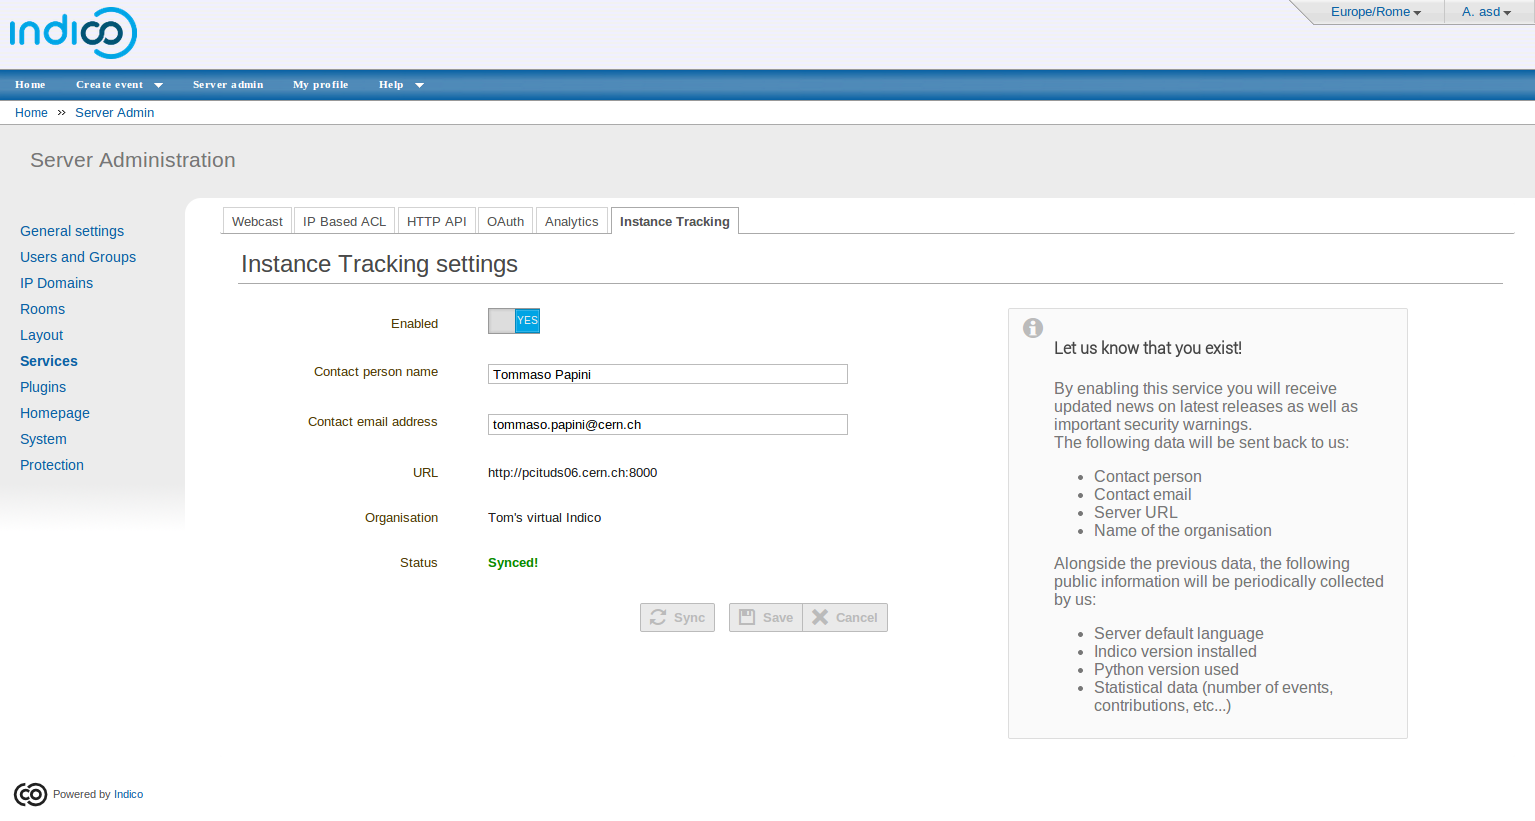
\includegraphics[scale=0.5]{indico_side.png}
    		\end{center}
    		\caption[Configurazione di Cephalopod in Indico]{Pagina amministrativa per la gestione delle opzioni di tracciamento in Indico.}
    		\label{fig:indico_side}
    	\end{figure}
    	
    	La voce ``Status'' indica se l'istanza è sincronizzata o meno con Cephalopod, ovvero se sono state fatte delle modifiche non ancora inviate a Cephalopod. Per implementare questo meccanismo viene fatta una richiesta \ac{HTML} da Indico all'\ac{API} di Cephalopod ``Get instance'': se l'istanza è registrata nel database di Cephalopod e i dati restituiti coincidono, allora l'istanza è sincronizzata, altrimenti no.
    	
    	Il pulsante ``Sync'' serve invece ad avviare la sincronizzazione tra istanza e Cephalopod. In particolare, se l'istanza non è presente nel database di Cephalopod, questa viene creata tramite l'\ac{API} ``Create instance'', altrimenti questa viene semplicemente aggiornata con i nuovi dati tramite l'\ac{API} ``Update instance''.
    	
    	Questa pagina serve sia come riepilogo dei dati principali scambiati con Cephalopod, sia per modificare e aggiornare gli stessi. Inoltre possiamo notare che accanto alla voce ``Enabled'' è presente un interruttore, che permette all'amministratore di attivare o disattivare in qualsiasi momento il tracciamento della propria istanza. Come già detto prima, questa è la scelta che è stata fatta dagli sviluppatori di Indico per il caso specifico di Indico: altri sviluppatori di un'altra applicazione potrebbero decidere di lasciare il tracciamento sempre abilitato di default, senza possibilità di disattivazione (anche se, per correttezza, sarebbe in ogni caso consigliabile avvertire gli utenti di tale scelta).
    	
    	Inoltre è stato aggiunto anche un avviso popup, non intrusivo, sulla pagina principale del pannello di amministrazione di Indico, che avverte l'amministratore se l'istanza è fuori sincronia con Cephalopod. L'amministratore potrà scegliere se sincronizzare l'istanza subito oppure ignorare l'avviso, che scomparirà dopo poco da solo. In Figura \ref{fig:admin_general} si può vedere come viene visualizzato tale messaggio.
    	
    	\begin{figure}[h!]
    		\begin{center}
    			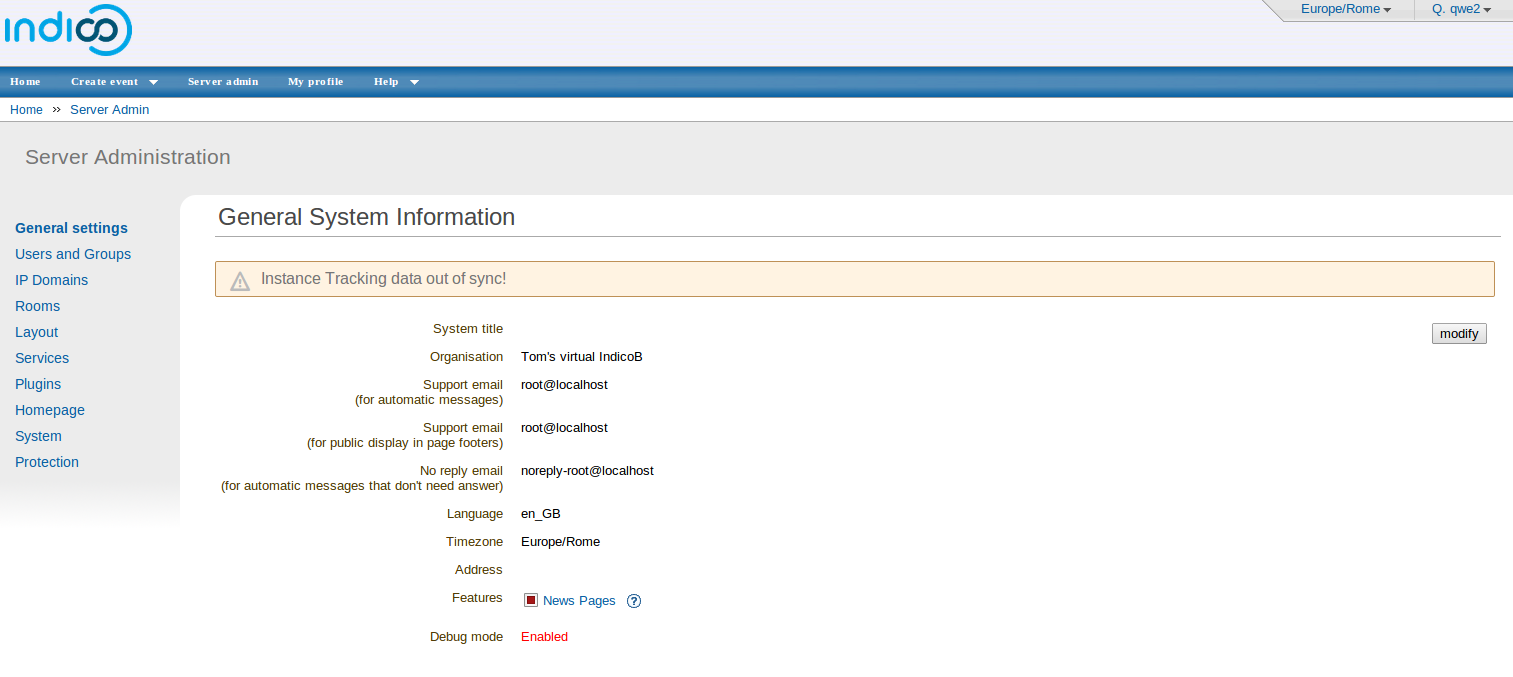
\includegraphics[scale=0.5]{admin_general.png}
    		\end{center}
    		\caption[Avviso della mancata sincronia con Cephalopod]{Avviso nella pagina principale di amministrazione di Indico che avverte della mancata sincronizzazione dell'istanza con Cephalopod.}
    		\label{fig:admin_general}
    	\end{figure}
    
        \subsection{Prima configurazione} \label{subsec:it;ai;prima_configurazione}
        
            L'ultima parte del processo di adattamento di Cephalopod a Indico riguarda la creazione di una pagina di prima configurazione per Indico.
            
            Dal momento che si è scelto di avvertire l'amministratore di un'istanza, fin da subito, della possibilità di poter attivare il servizio di tracciamento (mettendolo in grado di non attivarlo nemmeno mai, se non lo volesse) è risultato necessario dover porre tale domanda all'amministratore non appena l'istanza di Indico è stata installata ed è pienamente funzionante.
            
            L'idea era quella di mostrare una pagina dedicata, al posto della pagina principale di Indico, la prima volta in cui un amministratore effettuasse il primo accesso all'applicazione. Tuttavia creare una pagina apposita soltanto per una semplice domanda (``vuoi attivare il tracciamento? sì/no'') ci è sembrato un po' uno spreco, al momento, così è stato deciso di cogliere l'occasione per creare una vera e propria pagina di prima configurazione per Indico, dove venissero chieste le informazioni di base dell'amministratore e dell'istanza e che presentasse uno stile moderno e rinnovato, in pieno accordo con la filosofia del Progetto KT.
            
            Il risultato di questo lavoro è la pagina in Figura \ref{fig:initial_setup}.
            
        	\begin{figure}[h!]
        		\begin{center}
        			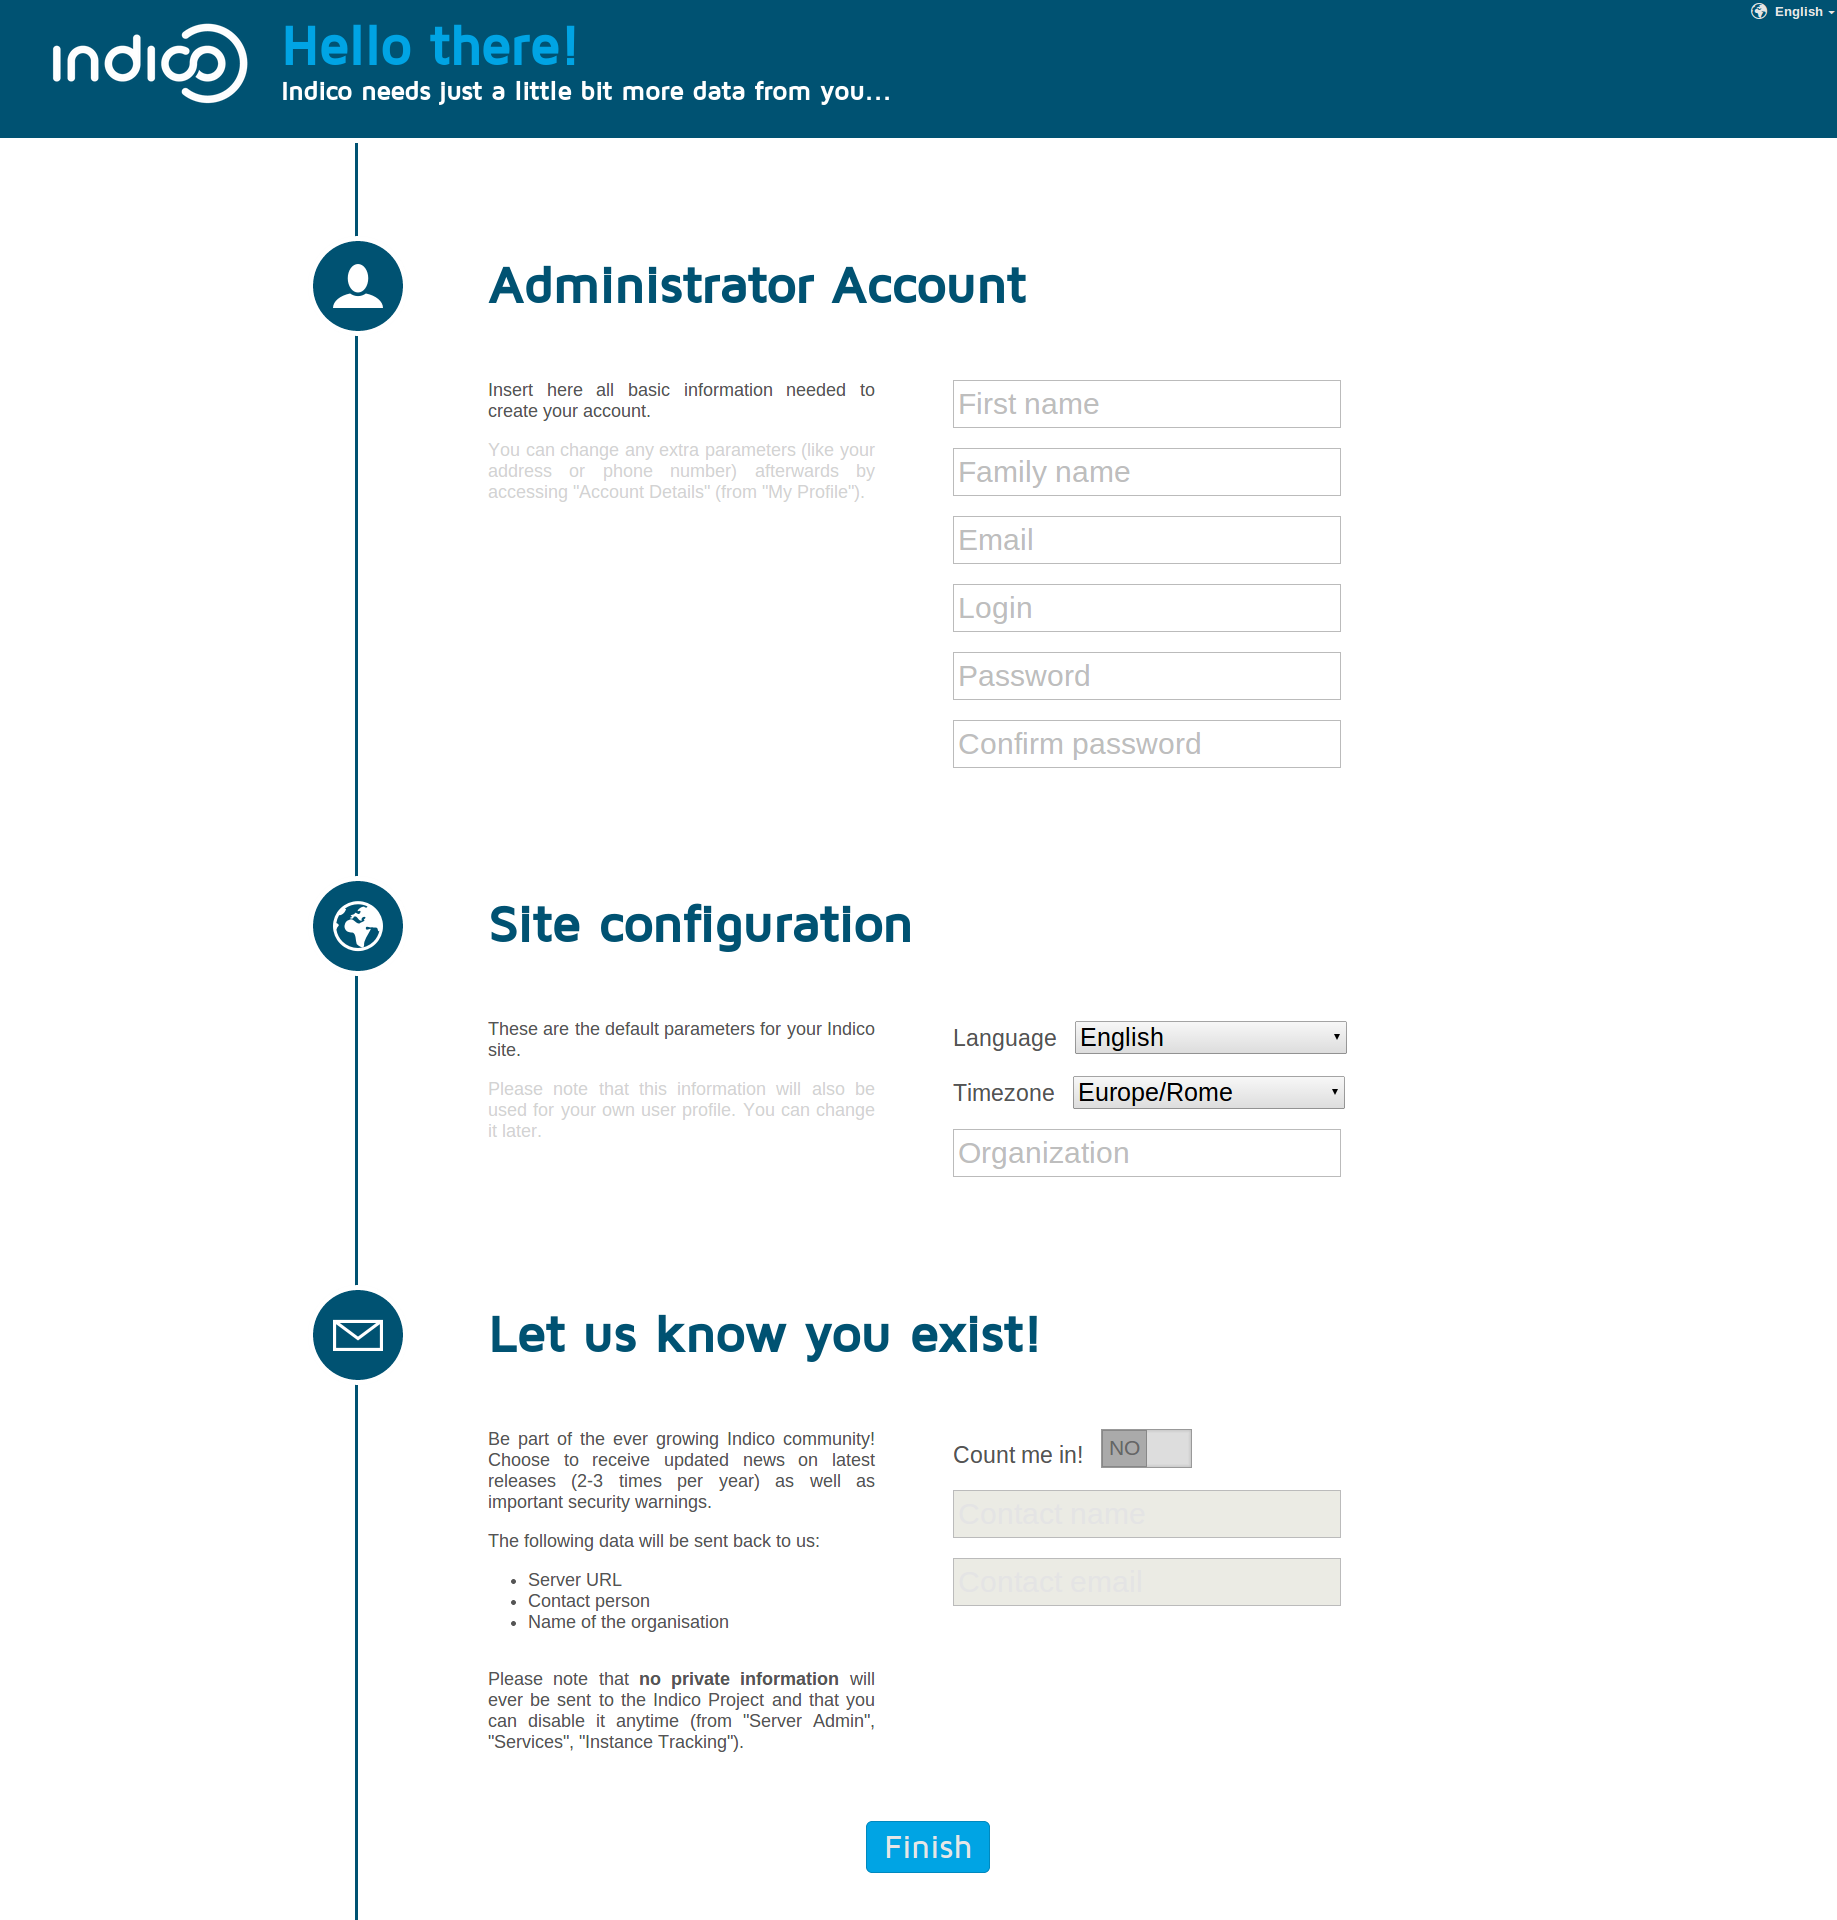
\includegraphics[scale=0.2]{initial_setup.png}
        		\end{center}
        		\caption[Prima configurazione di Indico]{Nuova pagina di prima configurazione per amministratori di Indico.}
        		\label{fig:initial_setup}
        	\end{figure}
        	
        	Come possiamo vedere, vengono richieste giusto alcune informazioni base e l'ultimo passo riguarda proprio il sistema di tracciamento, rendendo chiaro fin da subito cosa esso comporti e facendo scegliere l'amministratore se partecipare o meno.
    